\documentclass[a4paper,12pt,openany]{book}

\usepackage{ZeroSeven}
\usepackage{ltablex}
\usepackage{hyperref}
\titlepage{}

\author{Ludovico Brocca}
\date{2018-12-19}
\intestazioni{
\includegraphics[scale=0.3]{images/logo_intestazione}}
\pagestyle{myfront}
\begin{document}
\begin{titlepage}
	\centering
	{\huge\bfseries MegAlexa \par}
	Arricchitore di skill di Amazon Alexa
	\line(1,0){350} \\
	{\scshape\LARGE Manuale dello Sviluppatore \par}
	\vspace{1cm}
	{\scshape Gruppo ZeroSeven \par}
	\logo
	%devono essere compilati questi campi ogni volta
	\begin{tabular}{c|c}
		{\hfill \textbf{Versione}} 			& 0.0.5	\\
		{\hfill\textbf{Data Redazione}} 	& 2019-03-29	\\ 
		{\hfill\textbf{Redazione}} 			&  		Mirko Franco \\
		{\hfill\textbf{Verifica}} 				&  	?? \\
		{\hfill\textbf{Approvazione}} 		&  	?? \\
		{\hfill\textbf{Uso}} 					& 		Esterno		\\ 
		{\hfill\textbf{Distribuzione}} 			& 			Prof. Tullio Vardanega \\ & Prof. Riccardo Cardin \\ & Gruppo ZeroSeven	\\ & Zero12 s.r.l. \\
		{\hfill\textbf{Email di contatto}} & zerosevenswe@gmail.com \\
	\end{tabular}
\end{titlepage}
	
	\label{LastFrontPage}
	\newpage	
	\begin{center}
	\textbf{Registro delle modifiche}
	\end{center}
	\begin{center}
		\begin{tabularx}{\textwidth}{|c|c|X|X|c|}
			\hline
			\textbf{Versione} & \textbf{Data} & \textbf{Descrizione} & \textbf{Autore} & \textbf{Ruolo} \\ 
			\hline
			3.0.0 & 2019-04-11 & Approvazione per il rilascio RQ & Ludovico Brocca & Responsabile \\
			\hline
			2.1.0 & 2019-04-09 & Verifica documento & Ludovico Brocca & Verificatore \\
			\hline
			2.0.6 & 2019-04-08 & Aggiunto riferimento metriche alla sezione \S\ref{MetricheObbiettivi} &Matteo depascale & Amministratore \\
			\hline 
			2.0.5 & 2019-04-08 & Modifica sezioni \S\ref{Verifica}  e \S\ref{Validazione} & Matteo depascale & Amministratore \\
			\hline
			2.0.4 & 2019-04-08 & Aggiunti comandi personalizzati alla sezione \S\ref{NormeRedazionali} &Matteo depascale & Amministratore \\
			\hline
			2.0.3 & 2019-04-04 & Aggiunta voci a \S\ref{ListaControllo} & Matteo depascale & Amministratore \\
			\hline
			2.0.2 & 2019-04-01 & Stesura sezioni \S\ref{DiagrammiDelleClassi}, \S\ref{DiagrammiPackage}, \S\ref{DiagrammiSequenza} e \S\ref{DiagrammiAttivita}  & Bianca Andreea Ciuche & Amministratore \\
			\hline
			2.0.1 & 2019-03-23 & Modifica \ref{Documentazione fornita} Corretti numeri di sezione & Bianca Andreea Ciuche & Amministratore \\
			\hline
			2.0.0 &2019-03-07 & Approvazione per il rilascio & Gian Marco Bratzu& Responsabile\\
			\hline
			1.2.0 &2019-03-02 & Verifica documento &Andrea Deidda& Verificatore\\
			\hline
			1.1.2 &2019-02-13 &Stesura \S\ref{calcoloOre} &Ludovico Brocca& Amministratore\\
			\hline
			1.1.1 &2019-02-13 &Modifica\S \ref{anDinamica} &Ludovico Brocca& Amministratore\\
			\hline
			1.1.0 &2019-02-07 &Verifica \S\ref{processo}, \ref{metriche}, \S\ref{progettazione} &Gian Marco Bratzu& Verificatore\\
			\hline
			1.0.4 &2019-02-04&Stesura \S\ref{processo}&Ludovico Brocca& Analista\\
			\hline
			1.0.3 & 2019-02-03 & Modifica \S\ref{metriche} & Stefano Zanatta & Amministratore\\
			\hline
			1.0.2 & 2019-02-02 & Stesura \S\ref{metriche} & Bianca Andreea Ciuche & Amministratore\\
			\hline
			1.0.1 & 2018-01-12 & Stesura \S\ref{progettazione} & Mirko Franco & Amministratore \\
			\hline
			1.0.0 & 2018-01-09 & Approvazione per il rilascio & Stefano Zanatta & Responsabile\\
			\hline
			0.2.0 & 2018-12-29 & Verifica documento & Stefano Zanatta & Verificatore\\
			\hline
			0.1.0 & 2018-12-18 & Verifica \S\ref{PdS} & Mirko Franco & Verificatore\\
			\hline
			0.0.6 & 2018-12-21 & Modifica \S\ref{Intro} & Andrea Deidda & Amministratore\\
			\hline
			0.0.5 & 2018-12-17 & Stesura \S\ref{Po} & Ludovico Brocca & Amministratore\\
			\hline
			0.0.4 & 2018-12-16 & Stesura \S\ref{Pp} & Matteo Depascale & Amministratore\\
			\hline
			0.0.3 & 2018-12-16 & Stesura \S\ref{Intro} & Bianca Ciuche & Amministratore\\
			\hline
			0.0.2 & 2018-12-10 & Stesura \S\ref{PdS} & Gian Marco Bratzu & Amministratore\\	
			\hline
			0.0.1 & 2018-12-08 & Struttura documento  & Ludovico Brocca & Amministratore\\
			\hline
	\end{tabularx}
	\end{center}

\newpage
	\pagestyle{mymain}
	\tableofcontents
	\listoffigures
	\listoftables
	\chapter{Introduzione}
\label{introduzione}
\section{Scopo del documento}
Il \textit{Piano di Qualifica} ha lo scopo di definire gli obbiettivi di qualità che il gruppo perseguita per il proprio prodotto. Per ottenere tali obbiettivi è necessario un processo di verifica continua di ogni attività. Questo consente di rilevare e correggere le anomalie riscontrate tempestivamente.\\
Questo documento descrive nel dettaglio la qualità dei processi più vicini nel tempo e ad alto livello quelli più lontani, per poi essere aggiornato con nuovi contenuti ogni volta che il gruppo lo ritiene necessario.
\section{Scopo del prodotto}
Lo scopo del progetto è quello di sviluppare un applicativo Mobile in grado di creare delle routine personalizzate per gli utenti gestibili tramite\glossario{Alexa}di\glossario{Amazon}. L'obbiettivo è quello di creare\glossario{skill}in grado di avviare\glossario{workflow}creati dagli utenti fornendogli dei\glossario{connettori}.
\section{Glossario}
Al fine di evitare ogni ambiguità di linguaggio e massimizzare la comprensione dei documenti, i termini tecnici, di dominio, gli acronimi e le parole che necessitano di essere chiarite, sono riportate nel \textit{Glossario v1.0.0}.\\
Ogni occorrenza di vocaboli presenti nel \textit{Glossario} è marcata da una "G" maiuscola in pedice.
\section{Riferimenti}
\subsection{Normativi}
\begin{itemize}
	\item  \textbf{Norme di Progetto}: \textit{Norme di Progetto v1.0.0};
	\item \textbf{Capitolato$_{G}$ C4}:\glossario{MegAlexa}: arricchitore di skill di Amazon Alexa.
	\item \textbf{Ciclo di Deming}
	\footnote{\url{https://it.wikipedia.org/wiki/Ciclo_di_Deming}}
\end{itemize}
\subsection{Informativi}\label{rfinf}
\begin{itemize}
	\item \textbf{Piano di Progetto}: \textit{Piano di Progetto v1.0.0};
	\item \textbf{Complessità ciclomatica}
	\item \textbf{Software Testing Fundamentals: Methods and Metrics} di Marnie L. Hutcheson, Wiley Publishing, Inc.  
	\footnote{\url{https://www.math.unipd.it/~tullio/IS-1/2018/Progetto/C4.pdf}}.
	
	
\end{itemize}

	\chapter{Requisiti di Sistema}
	\chapter{Procedura di installazione}

\section{Requisiti di Sistema}
\label{RequisitSistema}
\textit{MegAlexa} è composta da un'applicazione compatibile con la maggior parte dei dispositivi\glossario{Android}e da una skill Alexa.
\subsection{Applicazione}
L'applicazione è compatibile con tutti i dispositivi Android con versione 4.4 o superiore.
Per poter modificare e ampliare la app i seguenti requisiti devono essere soddisfatti:
\begin{itemize}

	\item \textbf{IDE Android Studio$_{G}$:} necessaria per eseguire e testare la app nel corso del suo sviluppo;
	\item \textbf{Git$_{G}$:} necessario per effettuare il \texttt{clone} della repository e il versionamento successivo del codice;
	\item \textbf{Gradle$_{G}$:} per il download automatico delle dipendenze e la compilazione del codice (consigliata versione 4.10.0 o superiore).

\end{itemize}


\subsection{Skill}
La skill è compatibile con tutti i dispositivi Amazon \textit{Echo$_{G}$}.

\section{Installazione App} \label{installazioneApp}
Per installare la app è obbligatorio seguire i seguenti passi:

\begin{enumerate}
	\item \textbf{Acquisire la repository:} eseguire il comando \texttt{git clone} seguito dal seguente URL: \textit{https://github.com/sgt390/ProgettoSweCodice.git};
	\item \textbf{Registrare il dispositivo:} accedere alla console di sviluppo offerta da amazon con le credenziali inviate dai membri del gruppo e registrare una key univoca per la applicazione denominata \textit{MegAlexa}\footnote{\url{https://developer.amazon.com/loginwithamazon/console/site/lwa/overview.html}};
	\item \textbf{Posizionamento della key:} una volta aperto Android Studio, creare una cartella nel percorso \texttt{/MegAlexa/app/src/main}, nominarla \texttt{assets}, creare un file di testo nominato \texttt{api\_key.txt} e posizionarlo nella cartella appena creata;
	\item \textbf{Gradle Sync:} a questo punto, se la procedura è stata eseguita correttamente, Gradle dovrebbe scaricare in automatico le dipendenze per l'avvio della app, nel caso in cui ciò non avvenga, eseguire il comando \texttt{./gradlew build} nella cartella di root del progetto;
	\item\textbf{Compilazione ed esecuzione:} la compilazione può avvenire mediante il comando \texttt{./gradlew build} oppure mediante la pressione dell'icona a forma di martello presente in alto su Android Studio (vedi figura \ref{martello}), l'esecuzione avviene alla pressione del tasto run presente nell'IDE(vedi figura \ref{martello}).\\
	Alla prima esecuzione verrà richiesta l'installazione di una versione Android per l'emulatore: scegliere l'opzione più gradita e continuare.\\
	In alternativa, è possibile eseguire l'applicazione su un dispositivo Android predisposto correttamente(per maggiori dettagli visitare \url{https://developer.android.com/training/basics/firstapp/running-app}). 

	
\end{enumerate}

\begin{figure} [H]
	\centering
	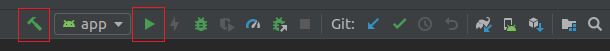
\includegraphics[scale=0.9]{./images/AndroidStudio.PNG}
	\caption{\textit{Tasti Build e Run}}\label{martello}
\end{figure}

\newpage
\section{Installazione Skill}
\label{installazioneSkill}
Per ognuno dei sequenti comandi è richiesta l'installazione del package manager \textbf{npm}.
Installazione della skill e delle sue dipendenze:
\begin{itemize}
    \item clonare la repository attraverso il comando \textit{git clone\\https://github.com/sgt390/MegAlexaSkill/};
    \item eseguire il comando \textit{npm install} per installare automaticamente le dipendenze.
\end{itemize}
Pubblicare la skill in AWS Lambda:
\begin{itemize}
    \item installare il programma \textit{7z$_{G}$} e inserire il suo eseguibile tra le variabili di sistema;
    \item installare e configurare aws-cli\footnote{\url{https://aws.amazon.com/it/cli/}};
    \item da terminal, eseguire il comando \textit{npm run publish-lambda}.
\end{itemize}
Eseguire i test di unità:
\begin{itemize}
    \item da terminal, eseguire il comando \textit{npm run unitTest}.
\end{itemize}
Eseguire i test di integrazione:
\begin{itemize}
    \item da terminal, eseguire il comando \textit{npm integrationTest}.
\end{itemize}

	\chapter{Tecnologie utilizzate}
\label{Tecnologie}
\section{Amazon Web Service}
Amazon Web Service è una piattaforma di cloud computing sicura che offre servizi di calcolo, memorizzazione, distribuzione di contenuti e altre funzionalità per aiutare il businesses ad essere scalabile e crescere con facilità. AWS fornisce infatti prodotti e servizi per costruire applicazioni, anche sofisticate, in modo flessibile, scalabile, economico e  con un'ottima resistenza ai guasti. 
\subsection{AWS DynamoDB}
Amazon DynamoDB è un database che supporta i modelli di dati di tipo documento e di tipo chiave-valore che offre prestazioni di pochi millisecondi a qualsiasi livello. Si tratta di un database multi master, multi regione e completamente gestito che offre sicurezza integrata, backup, ripristino e cache in memoria per applicazioni Internet. DynamoDB può gestire oltre 10 trilioni di richieste al giorno e supporta picchi di oltre 20 milioni di richieste al secondo. 
\subsection{AWS Lambda}
AWS Lambda consente di eseguire codice senza dover effettuare il provisioning né gestire il server. Le tariffe sono calcolate in base ai tempi di elaborazione.\\ 
Con Lambda, è possibile eseguire codice per qualunque tipo di applicazione o di servizio back-end, senza alcuna amministrazione. Una volta caricato il codice Lambda si prende carico delle azioni necessarie per eseguirlo e ricalibrarne le risorse con la massima disponibilità. \'E possibile configurare il codice in modo che venga attivato automaticamente da altri servizi AWS oppure che venga richiamato direttamente da qualsiasi app Web o mobile.
\subsection{AWS API Gateway}
AWS API Gateway è un servizio completamente gestito che semplifica la creazione, la pubblicazione, la manutenzione e la protezione delle API su larga scala. Con semplicità è possibile creare e configurare API REST che fungano da "porta di ingresso" per le applicazioni, per consentire l'accesso ai dati, alla logica di business o alle funzionalità dai propri servizi back-end. API Gateway gestisce tutte le attività di accettazione ed elaborazione relative a centinaia di migliaia di chiamate ad API simultanee, inclusi gestione del traffico, controllo di accessi e autorizzazioni, monitoraggio e gestione delle versione delle API. Gateway non prevede alcuna tariffa minima né investimenti iniziali. Vengono addebitati solo i costi di chiamate API ricevute e i volumi di dati trasferiti in uscita e con il modello tariffario a scaglioni di API Gateway potrai ridurre i costi al variare dell'utilizzo delle API.
\subsection{AWS CloudWatch}
AWS CloudWatch è un servizio di monitoraggio e gestione creato per gli sviluppatori, operatori di sistema, ingegneri responsabili del sito e manager IT. CloudWatch fornisce dati e analisi concrete per monitorare le applicazioni, capire e rispondere ai cambiamenti di prestazioni a livello di sistema, ottimizzare l'utilizzo delle risorse e ottenere una visualizzazione unificata dello stato di integrità operativa. 
\subsection{Node.js}
La skill è sviluppata attraverso un progetto Node js. Tutte le classi (apparte index.js) sono scritte in Typescript, ma vengono compilate in Javascript prima di essere trasferite in AWS Lambda.
\subsection{Npm}
Gestore di package per node.js. Permette l'esecuzione di comandi personalizzati (come descritto in \S\ref{installazioneSkill}).
\subsection{7z}
Permette di comprimere i file da linea di comando. \`{E} richiesto dalla procedura di build della skill.

\section{Dipendenze esterne}

\subsection{Alexa Skill}\label{ATecnologie}
Tutte le dipendenze principali si trovano nel file \textit{package.json}, mentre quelle secondarie (cioè le dipendenze delle dipendenze) stanno nel file package-lock.json.\\
Dipendenze principali:
\begin{itemize}
    \item \textbf{ask-sdk:} (Alexa Skill Kit) permette di comunicare direttamente con i servizi Amazon Alexa;
    \item \textbf{axios:} chiamate HTTP. Utilizzato principalmente in WorkflowService per le chiamate REST e nei connettori;
    \item \textbf{openweather-apis:} informazioni riguardanti il tempo atmosferico;
    \item \textbf{rss-parser:} trasformazione di un file RSS in un testo più leggibile;
    \item \textbf{twitter:} comunicazione con i servizi Twitter.
\end{itemize}
Dipendenze utili solo allo sviluppatore (test e compilazione):
\begin{itemize}
    \item \textbf{mocha:} framework per i test in Javascript;
    \item \textbf{chai:} funzionalità aggiuntive mocha;
    \item \textbf{@types/node:} definizioni dei tipi di Node.js per Typescript;
    \item \textbf{@types/mocha:} adattatore mocha per Typescript; 
    \item \textbf{@types/chai:} adattatore chai per Typescript;
    \item \textbf{@types/chai-as-promised:} dipendenza aggiuntiva di chai per valutare le \textit{promise};
    \item \textbf{typescript:} permette la compilazione da Typescript a Javascript.
\end{itemize}

\subsection{App Android}
	\chapter{Architettura}
\section{Skill}\label{architetturaSkill}
La skill è hostata nel sito https://developer.amazon.com/alexa/ (è necessario un account developer Amazon per accedervi). La skill è rappresentata da un JSON, configurabile attraverso l'UI fornito dalla piattaforma Alexa developer.
\begin{figure} [H]
    \centering
	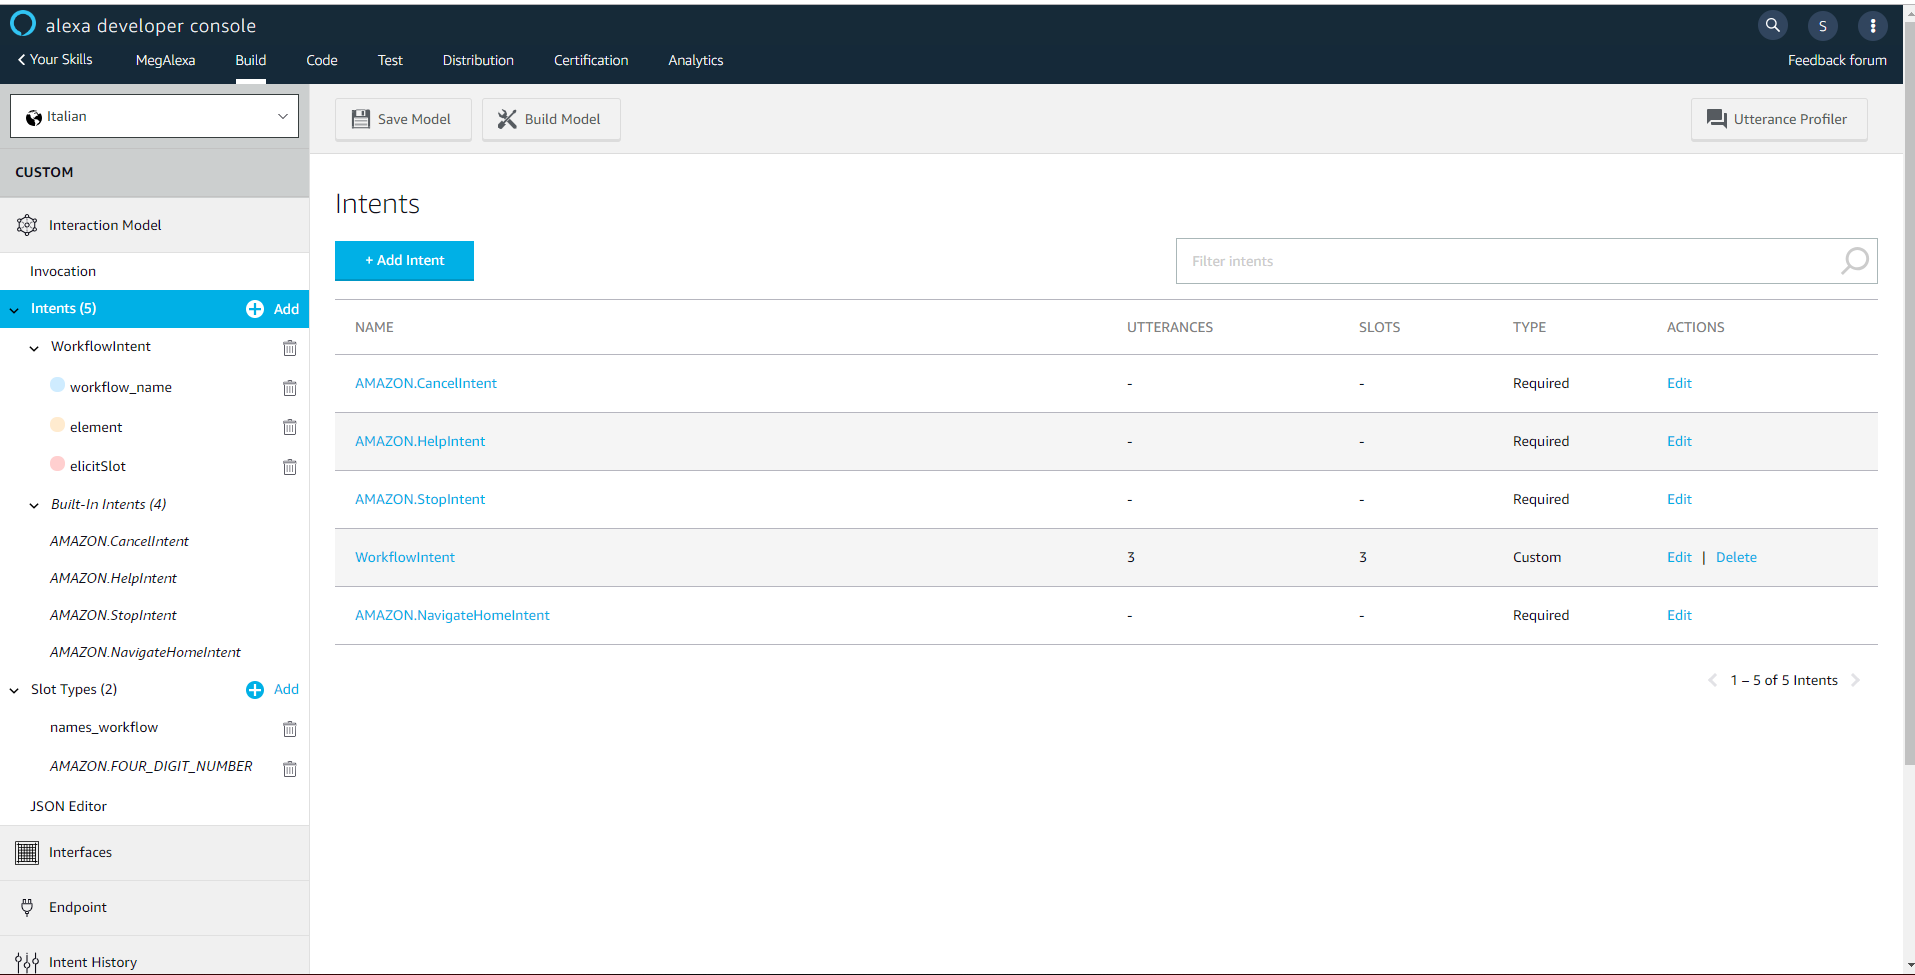
\includegraphics[scale=0.2]{./images/SkillPage.PNG}
	\caption{\textit{Alexa developer platform}}\label{classlambda}
\end{figure}


La logica della skill è hostata in una AWS Lambda, quindi è serverless. Questo significa che viene creata una nuova istanza della Skill ogni volta che arriva una richiesta da Alexa (ogni utente genera una istanza diversa). L'architettura della Skill si basa sul concetto di avere una skill leggera, che esegue poche operazioni ogni volta che questa viene invocata.\\
Una richiesta da parte di Alexa viene catturata dall'index, che la elabora e ritorna un risultato. Una richiesta è definita da un JSON contenente molteplici informazioni sullo stato del dialogo, l'utente, errori e molto altro. Una dettagliata descrizione si trova sulla documentazione di Amazon AWS\footnote{\url{https://developer.amazon.com/docs/custom-skills/request-and-response-json-reference.html}}.\\
Le informazioni più importanti contenute nel file JSON sono:\label{paramsSkill}
\begin{itemize}
    \item \textbf{handlerInput.requestEnvelope.request.type:} rappresenta il tipo di richiesta: IntentRequest o LaunchRequest. LaunchRequest rappresenta la prima iterazione con la skill ("Alexa, apri MegAlexa"), IntentRequest rappresenta tutte le altre richieste;
    \item \textbf{handlerInput.requestEnvelope.request.intent.name:} contiene il nome della richiesta, definiti dove la skill viene hostata. I casi più comuni sono "WorkflowIntent", "StopIntent" e "HelpIntent";
    \item \textbf{handlerInput.requestEnvelope.request.slots:} contiene una lista di slot, cioè dei parametri che l'utente deve dire per continuare con il dialogo con Alexa;
    \item \textbf{handlerInput.requestEnvelope.request.attributesManager:} permette la gestione degli attributi di sessione. Servono per salvare delle variabili da una chiamata all'altro della skill (lambda).
\end{itemize}

Il seguente diagramma dei package descrive le dipendenze ad alto livello della Skill.\\
\begin{figure} [H]
    \centering
	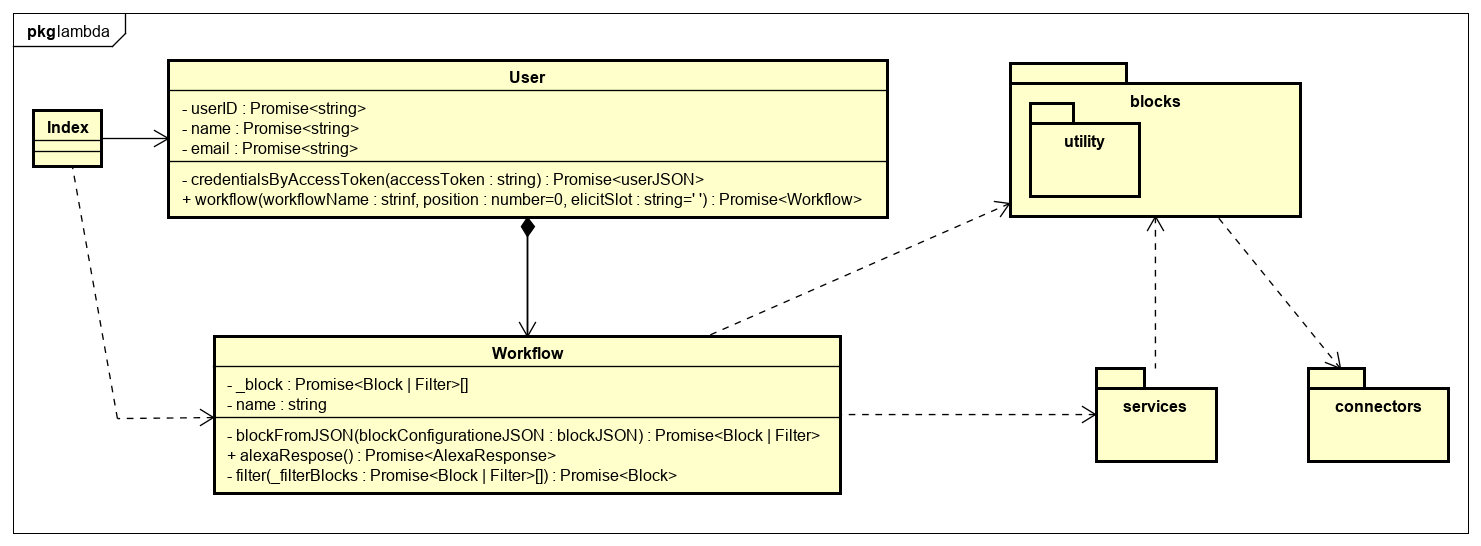
\includegraphics[scale=0.35]{./images/ZeroSevenPackageLambda.png}
	\caption{\textit{Skill class diagram}}\label{classlambda}
\end{figure}
\clearpage
La classe \textit{User} rappresenta un singolo utente che sta utilizzando la skill. L'utente usa la classe \textit{WorkflowService} per creare un \textit{Workflow}. \textit{Workflow} crea una lista di \textit{Block}. Alcuni \textit{Block} creano un \textit{connector} per fare chiamate HTTP.\\
I blocchi che devono fare chiamate HTTP, vengono rappresentati come delle Promise, per questo motivo anche \textit{Workflow} viene rappresentato in una promise in \textit{User}.\\
Tutte le classi sono scritte in TypeScript. L'index è scritto in Javascript (per compatibilità con ask-sdk). Prima di fare il deploy in AWS Lambda, i file TypeScript vengono compilati in Javascript.
\subsection{Index}
Index contiene gli handler, funzioni che catturano le richieste da parte di Alexa. Tutti gli handler sono definiti nella funzione "handler", e vengono eseguiti nell'ordine di dichiarazione.\\Ogni singolo handler è formato da due parti:
\begin{itemize}
    \item canHandle: verifica se quello è il giusto handler da eseguire. Il controllo viene fatto usando i parametri definiti in \S\ref{paramsSkill}. Se nessun handler può gestire la richiesta, viene invocato Error handler;
    \item handle: se canHandle ritorna True, questa è la funzione che viene eseguita. deve ritornare una risposta comprensibile da Alexa.
\end{itemize}
\subsection{Classe User}
In \textit{User} sono presenti i seguenti metodi:
\begin{itemize}
    \item \textbf{credentialsByAccessToken:} prende come parametro un access token (fornito da Amazon Alexa) e ritorna una Promise contenente un JSON, il quale contiene username, email e userID. Lo userID è lo stesso di quello ottenuto attraverso il collegamento dell'applicazione all'applicazione Android, permettendo di autenticare l'utente nel database;
    \item \textbf{Workflow:} usa WorkflowService per creare un Workflow a partire dalla sua rappresentazione in formato JSON.
\end{itemize}
\begin{figure} [H]
    \centering
	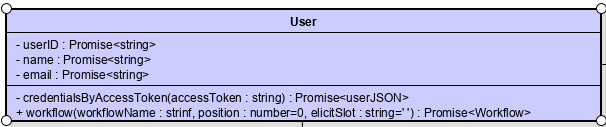
\includegraphics[scale=0.8]{./images/user.PNG}
	\caption{\textit{Skill class diagram - User}}\label{classlambda}
\end{figure}
\subsection{Classe Workflow}
In \textit{Workflow} sono presenti i seguenti metodi:
\begin{itemize}
    \item \textbf{blockFromJSON:} crea un blocco a partire dalla sua rappresentazione in JSON;
    \item \textbf{alexaResponse:} crea la risposta sotto forma di Promise<string> a partire dalle risposte di ogni blocco;
    \item \textbf{filter:} rimuove tutti i \textit{Filter} dalla lista di blocchi, e filtra i \textit{Block} (chiamando l'apposito metodo nel \textit{Block}) che seguono direttamente ogni Filter. Questo metodo non genera side effect.
\end{itemize}
\begin{figure} [H]
    \centering
	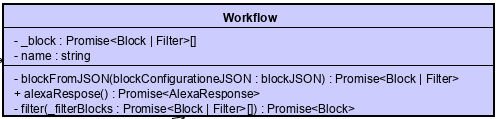
\includegraphics[scale=0.8]{./images/workflow.PNG}
	\caption{\textit{Skill class diagram - Workflow}}\label{classlambda}
\end{figure}
\subsection{Package services}
Il package services contiene la classe WorkflowService, che si occupa di creare un \textit{Workflow}, dopo aver ottenuto la sua rappresentazione JSON dal database (con una chiamata REST).
\begin{figure} [H]
    \centering
	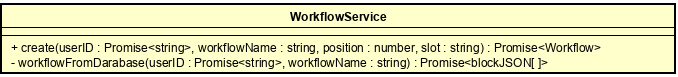
\includegraphics[scale=0.7]{./images/WorkflowService.PNG}
	\caption{\textit{Skill class diagram - WorkflowService}}\label{classlambda}
\end{figure}
\clearpage
\subsection{Package blocks}
Il package blocks contiene tutti i blocchi della skill e il package utils.\\
I blocchi implementano tutti l'interfaccia \textit{Block}, alcuni implementano anche \textit{Filterable} e \textit{ElicitBlock}.\\
Un blocco Filterable può essere rappresentato come una lista, quindi deve permettere di ritornare una versione di se stesso con meno elementi.\\
Un blocco ElicitBlock richiede all'utente dei parametri aggiuntivi per poter eseguire.
\begin{figure} [H]
    \centering
	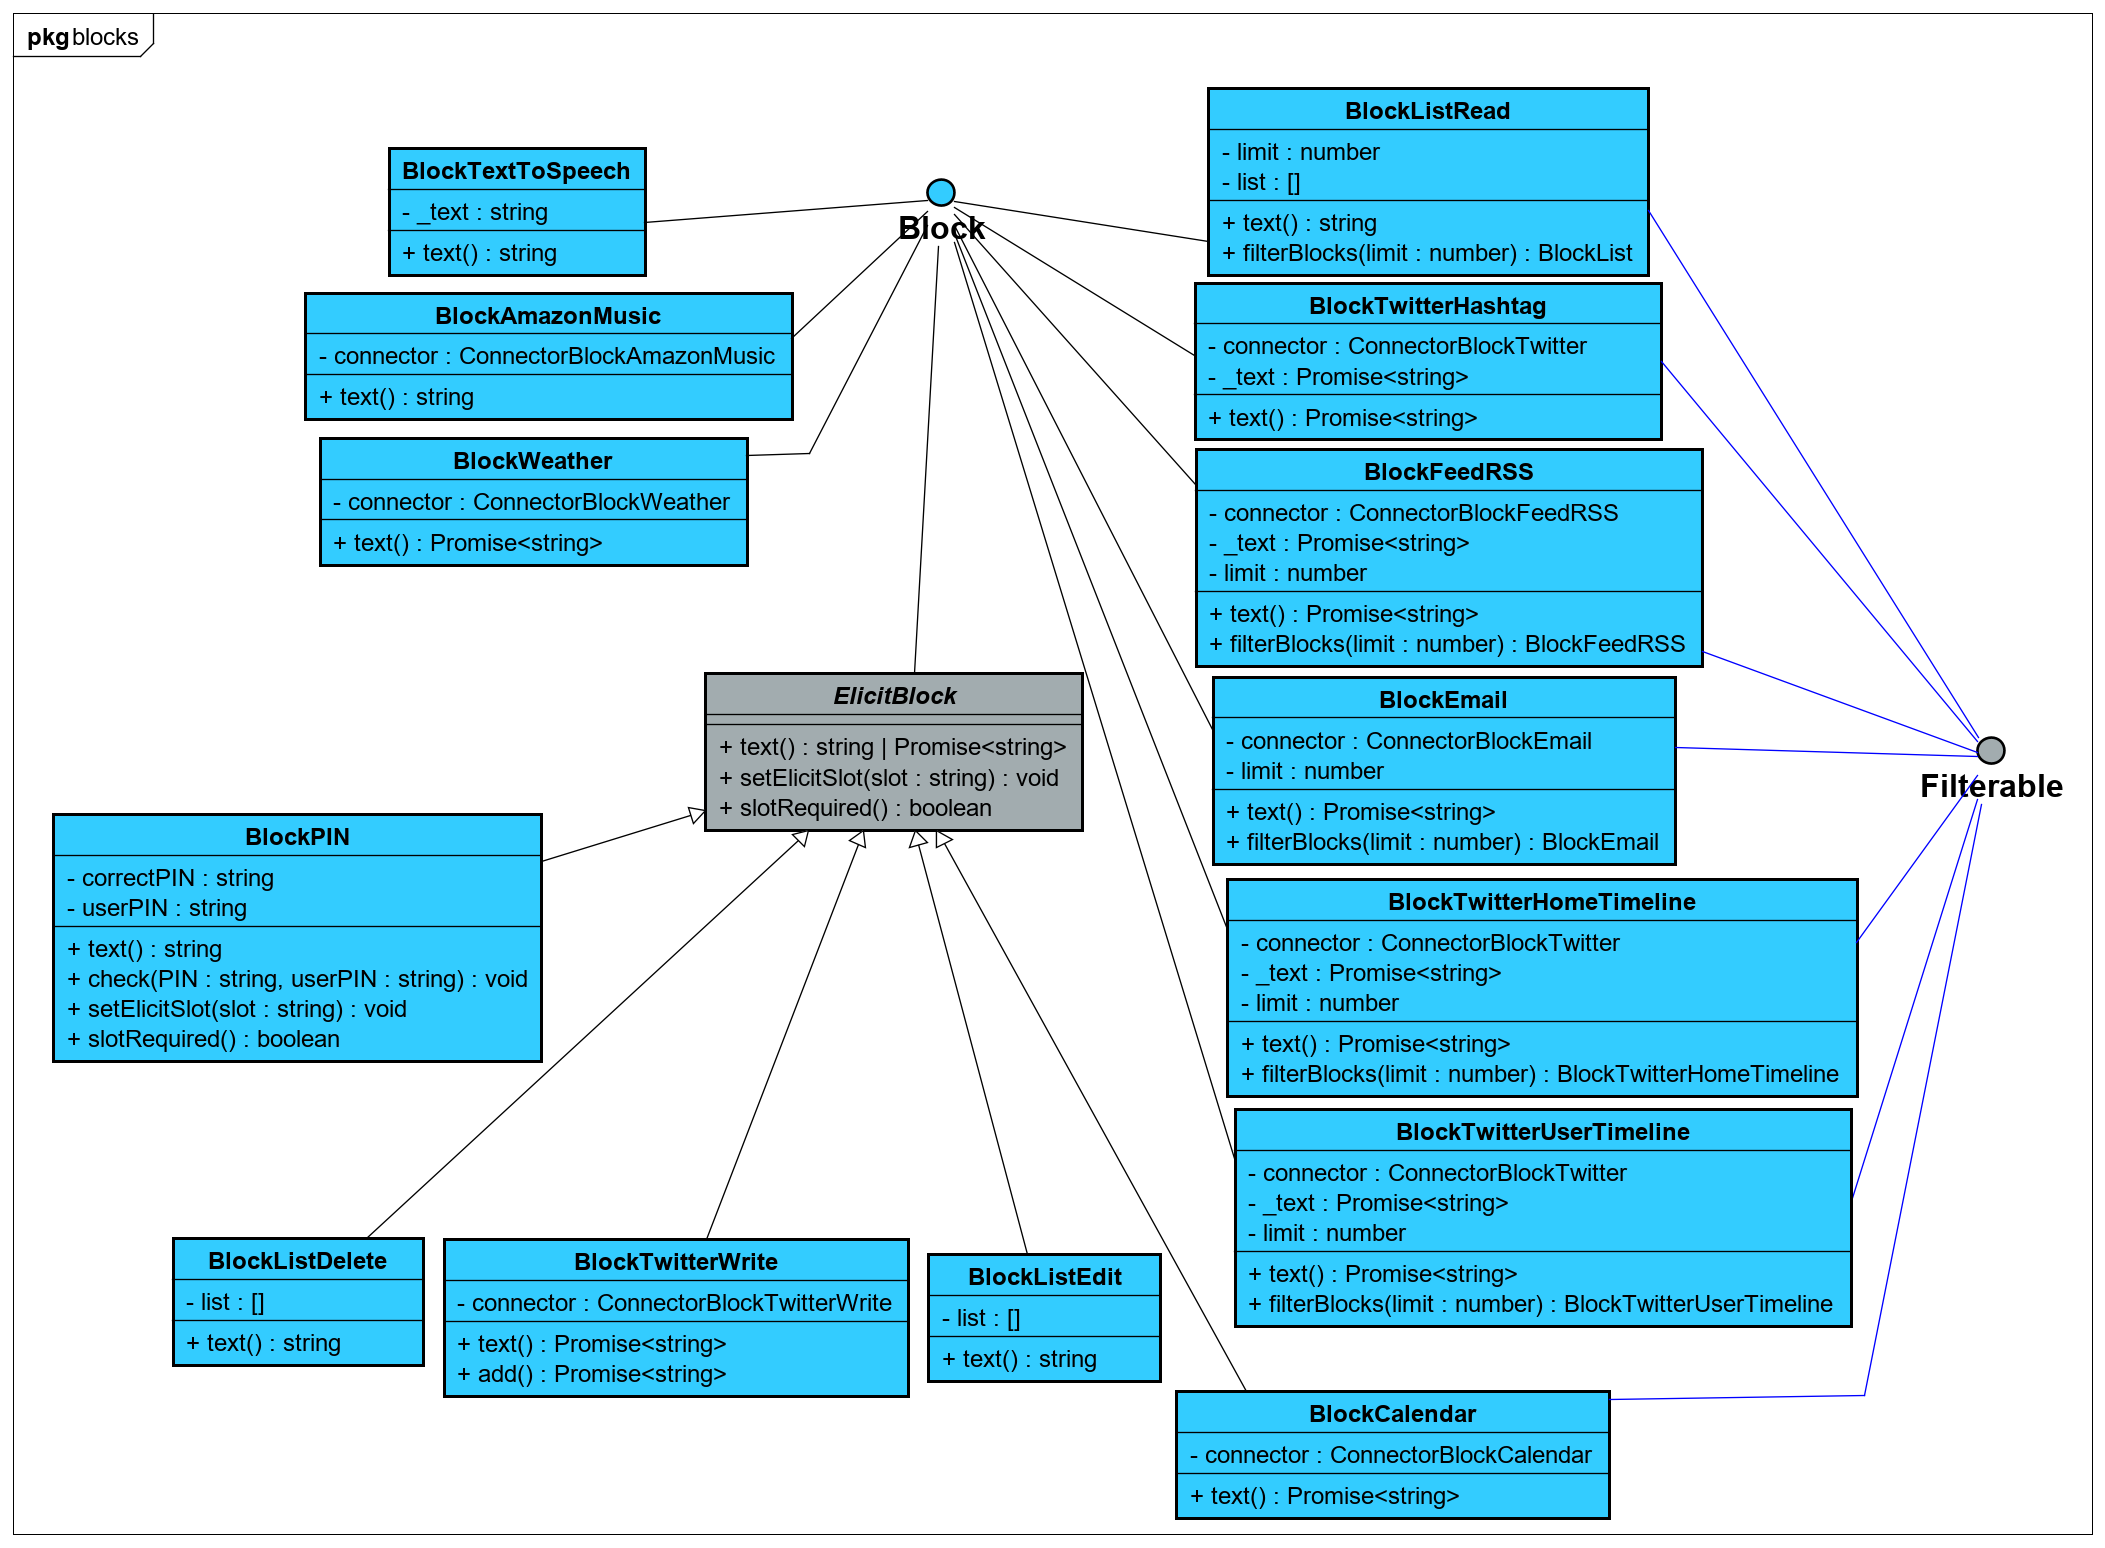
\includegraphics[scale=0.24]{./images/ZeroSevenClassBlocks.png}
	\caption{\textit{Skill class diagram - blocks package}}\label{classlambda}
\end{figure}
\subsubsection{Package blocks.utils}
Il package \textit{blocks.utils} contiene le interfacce utili ai \textit{Block} (ElicitBlock e Filterable).
\subsection{Package connectors}
Il package connectors contiene i connettori utilizzati dai blocchi.\\
Un Connector permette al blocco di ottenere le informazioni che gli servono da internet. Per esempio, BlockWeather (un blocco che rappresenta il meteo) chiamerà una liberia per conoscere il meteo di una certa zona.\\
Ogni Connector deve processare il risultato e trasformarlo nel testo che Alexa dovrà ripetere.
\begin{figure} [H]
    \centering
	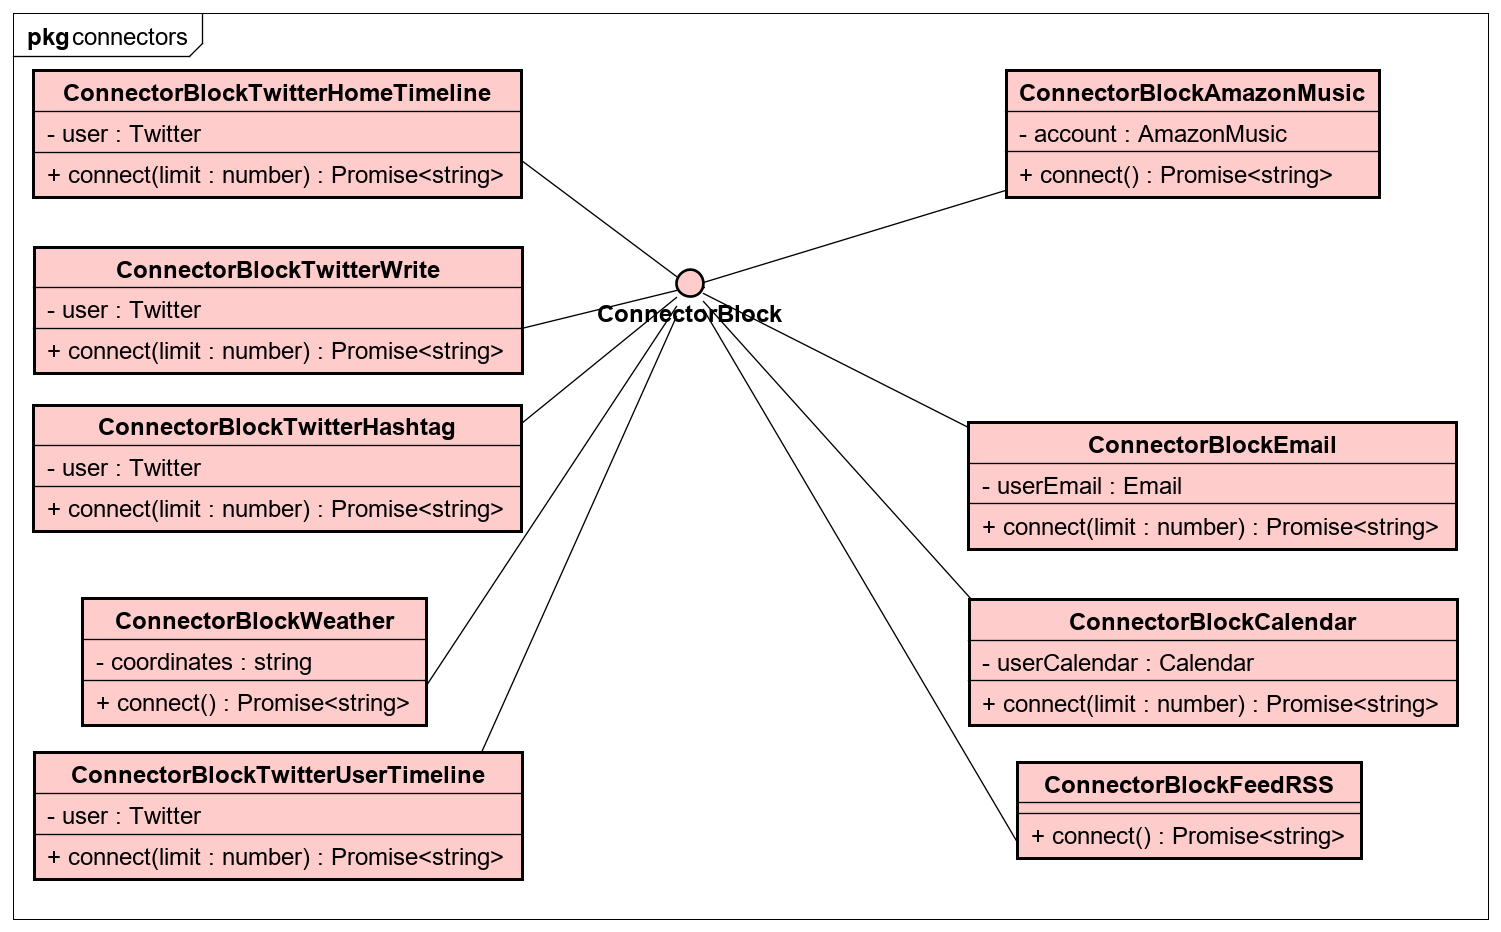
\includegraphics[scale=0.3]{./images/ZeroSevenClassConnectors.png}
	\caption{\textit{Skill class diagram - blocks package}}\label{classlambda}
\end{figure}

\newpage
\section{App}\label{architetturaApp}

L'app è hostata nella repository github https://github.com/sgt390/ProgettoSweCodice.
I pattern che abbiamo utilizzato sono:
\begin{itemize}
	\item \textbf{ModelViewViewModel} utilizzato per la gestione e scambio dati tra Model e View;
	\item \textbf{Builder} utilizzato per il Model (Workflow);
	\item \textbf{Singleton} utilizzato per il Model (Workflow);
	\item \textbf{Facade} utilizzato per le connessioni ad API esterne;
	\item \textbf{Strategy} utilizzato per il service;
	\item \textbf{Template Method} utilizzato per il service;
	
	
\end{itemize}


\begin{figure} [H]
	\centering
	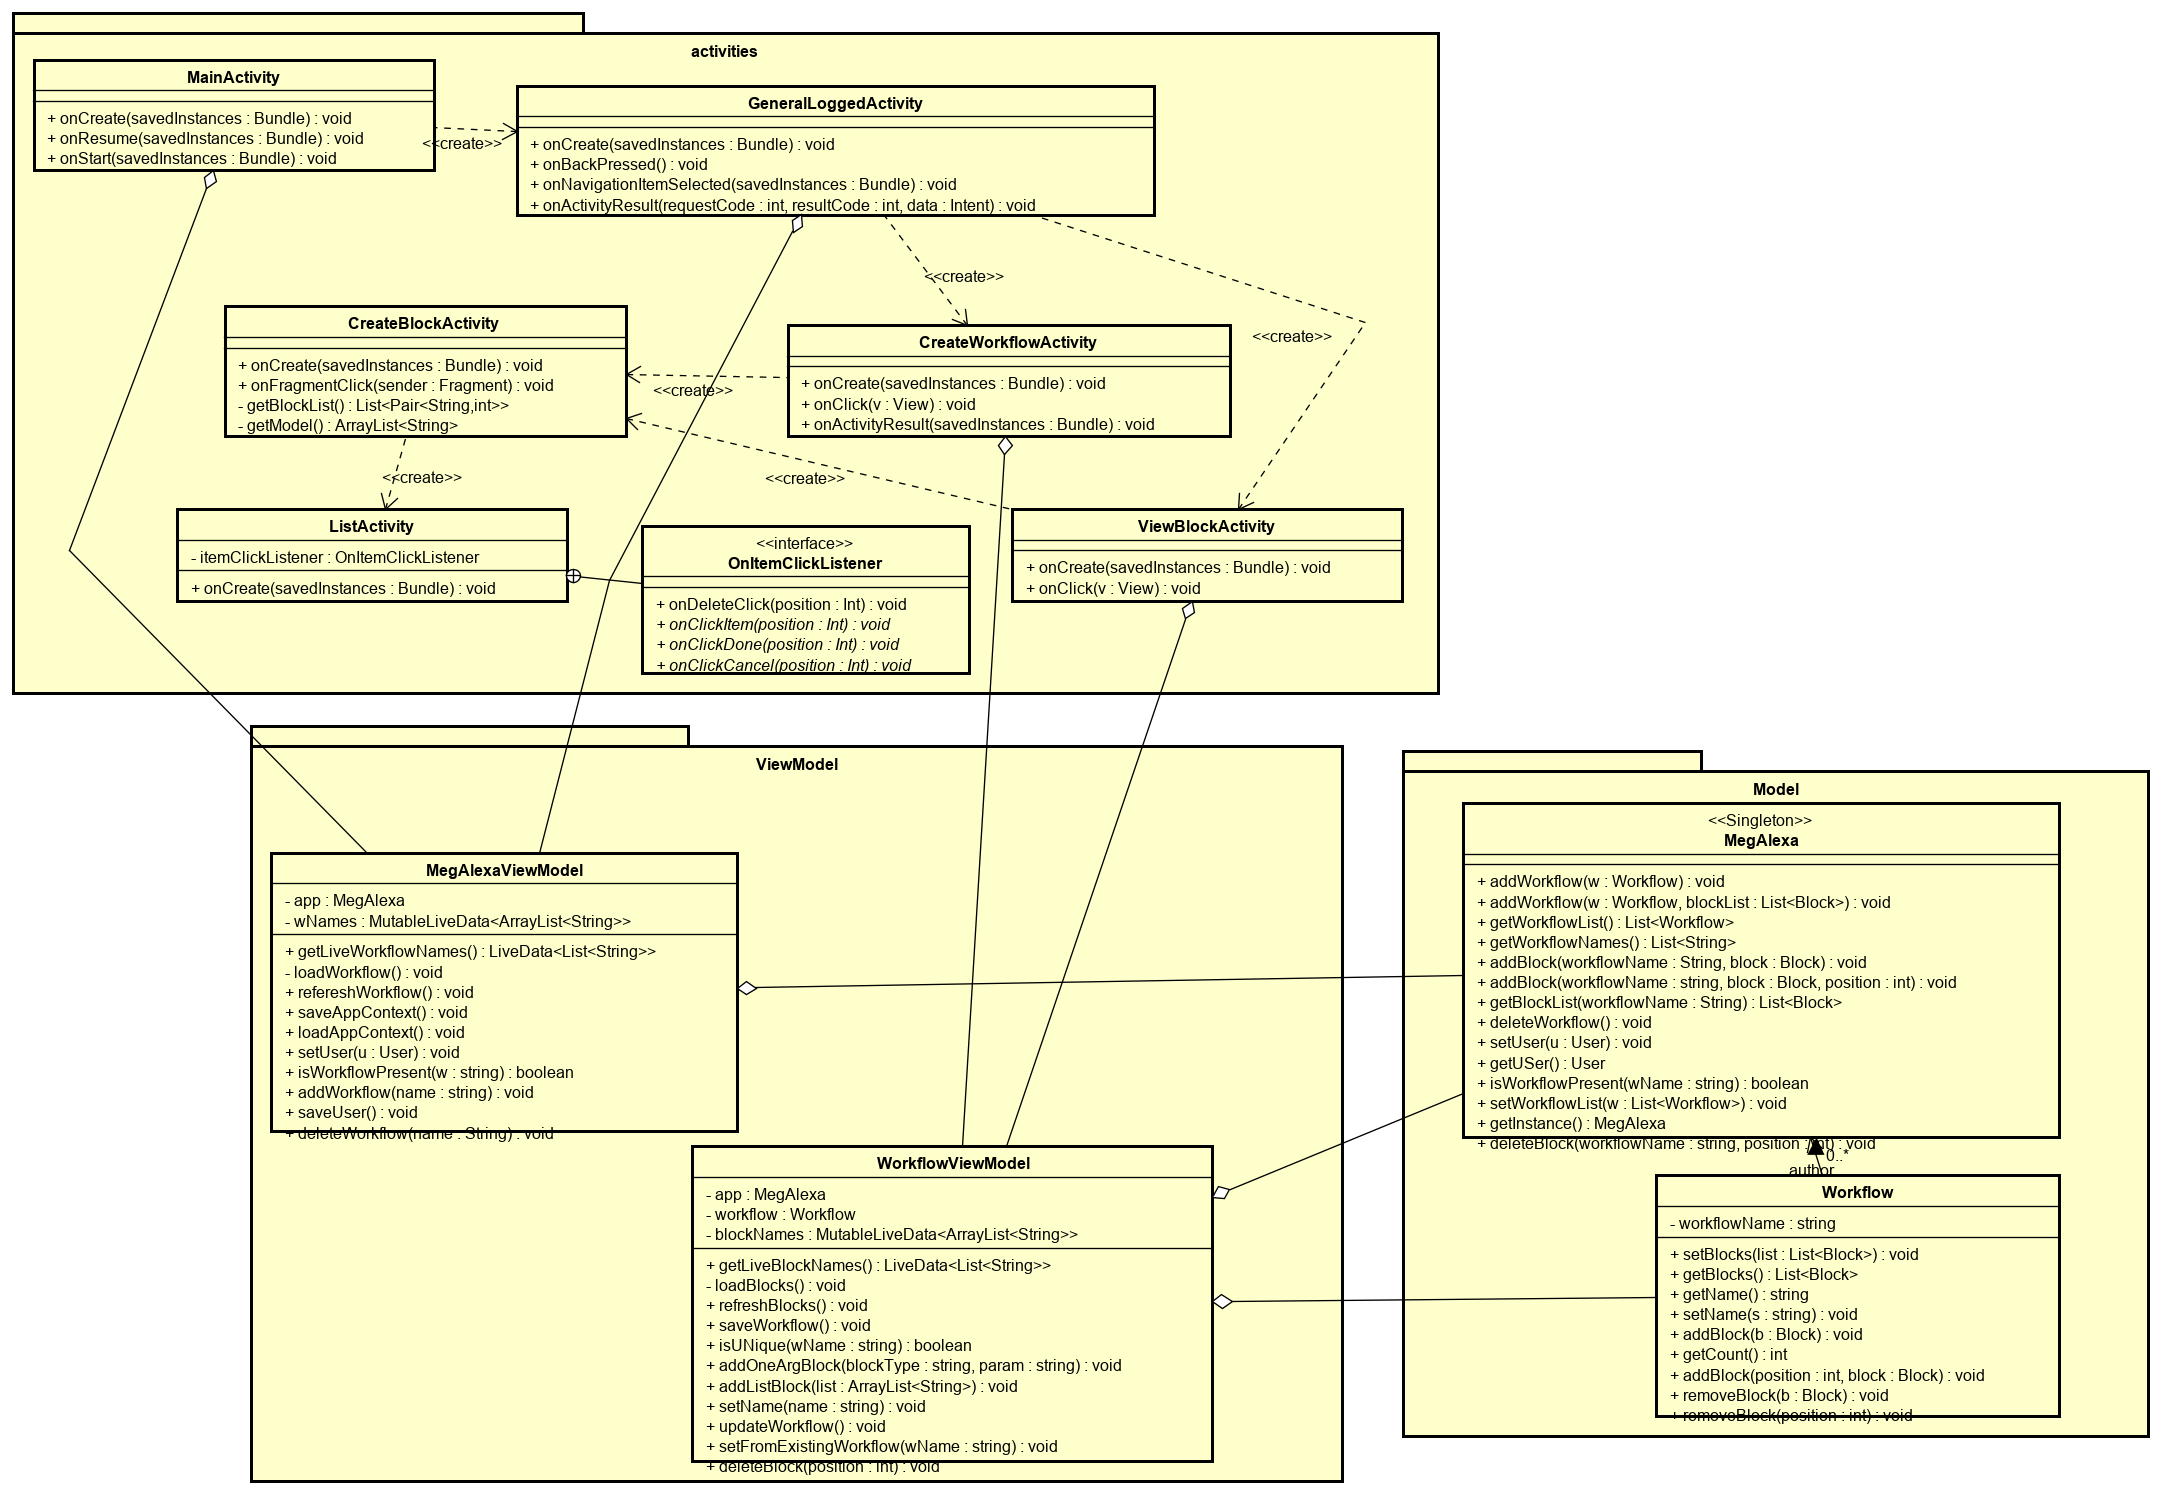
\includegraphics[scale=0.3]{./images/MVVM.png}
	\caption{\textit{App class diagram - MVVM}}\label{MVVM}
\end{figure}

\begin{figure} [H]
	\centering
	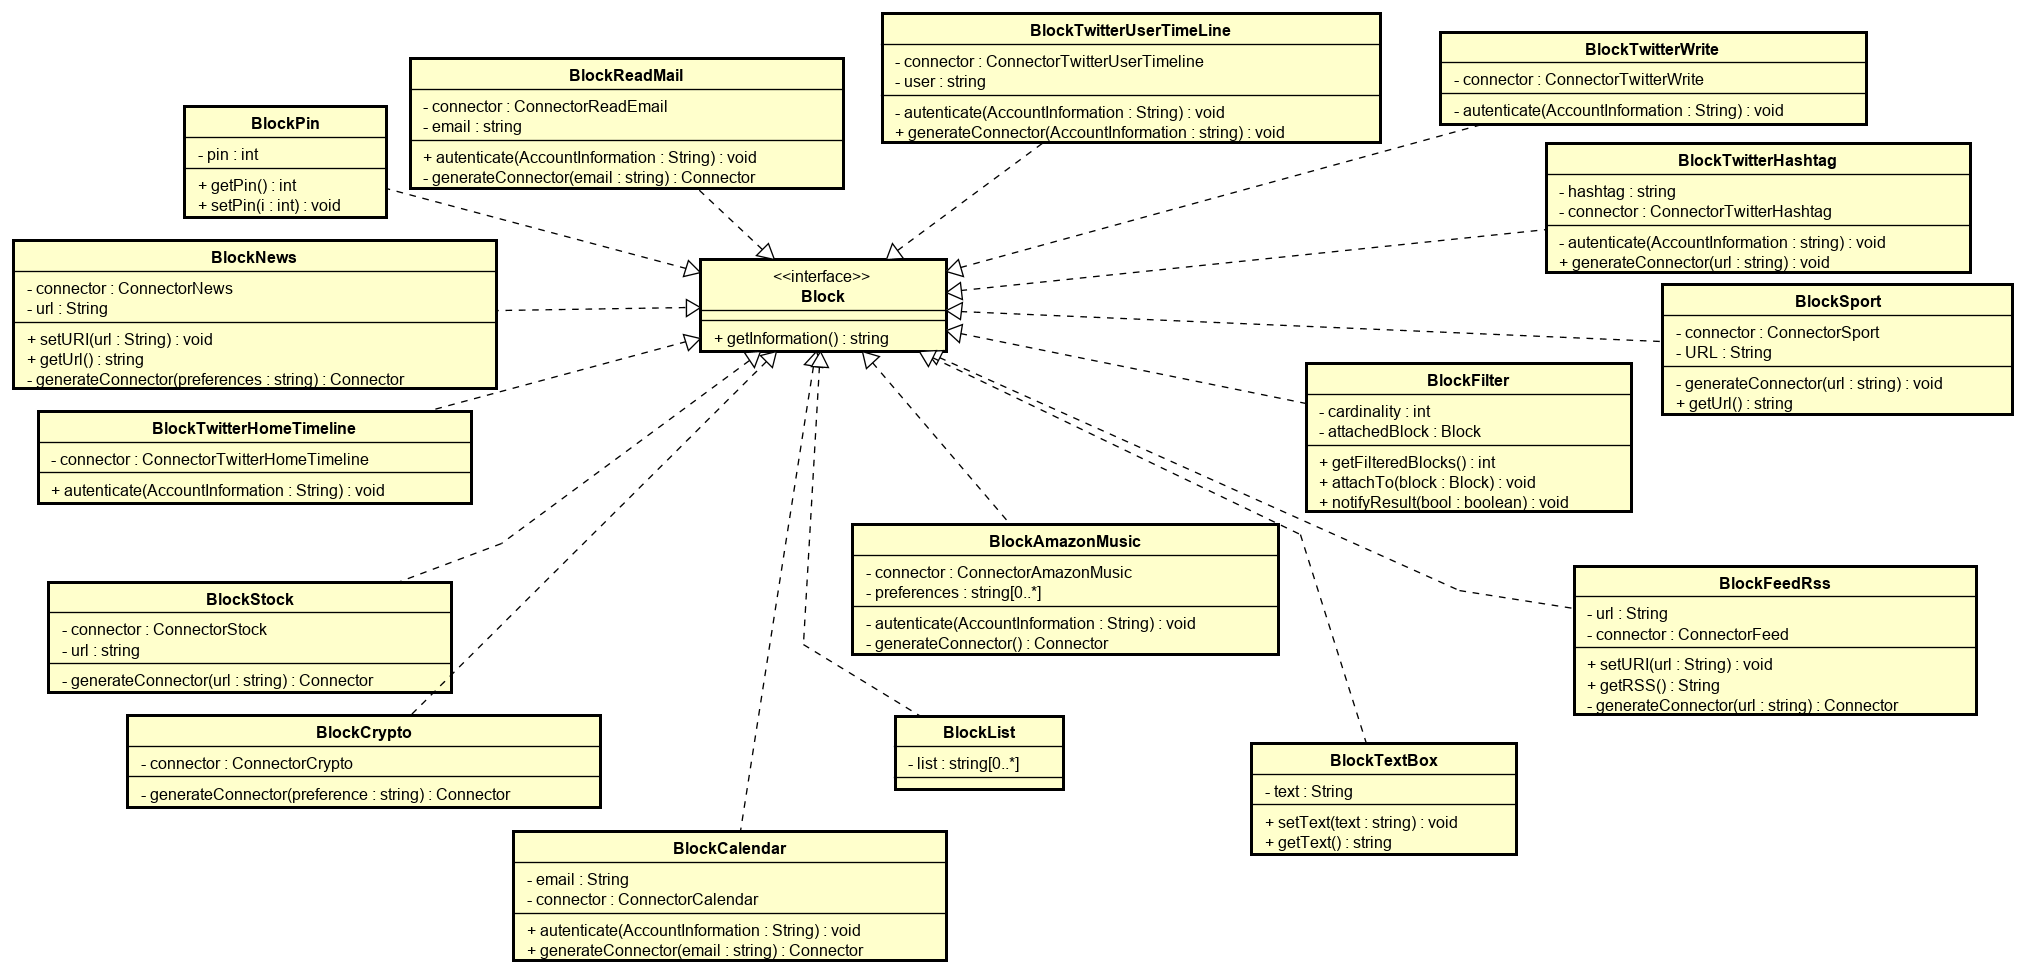
\includegraphics[scale=0.3]{./images/Blocks.png}
	\caption{\textit{App class diagram - Blocks}}\label{Blocks}
\end{figure}
\begin{figure} [H]
	\centering
	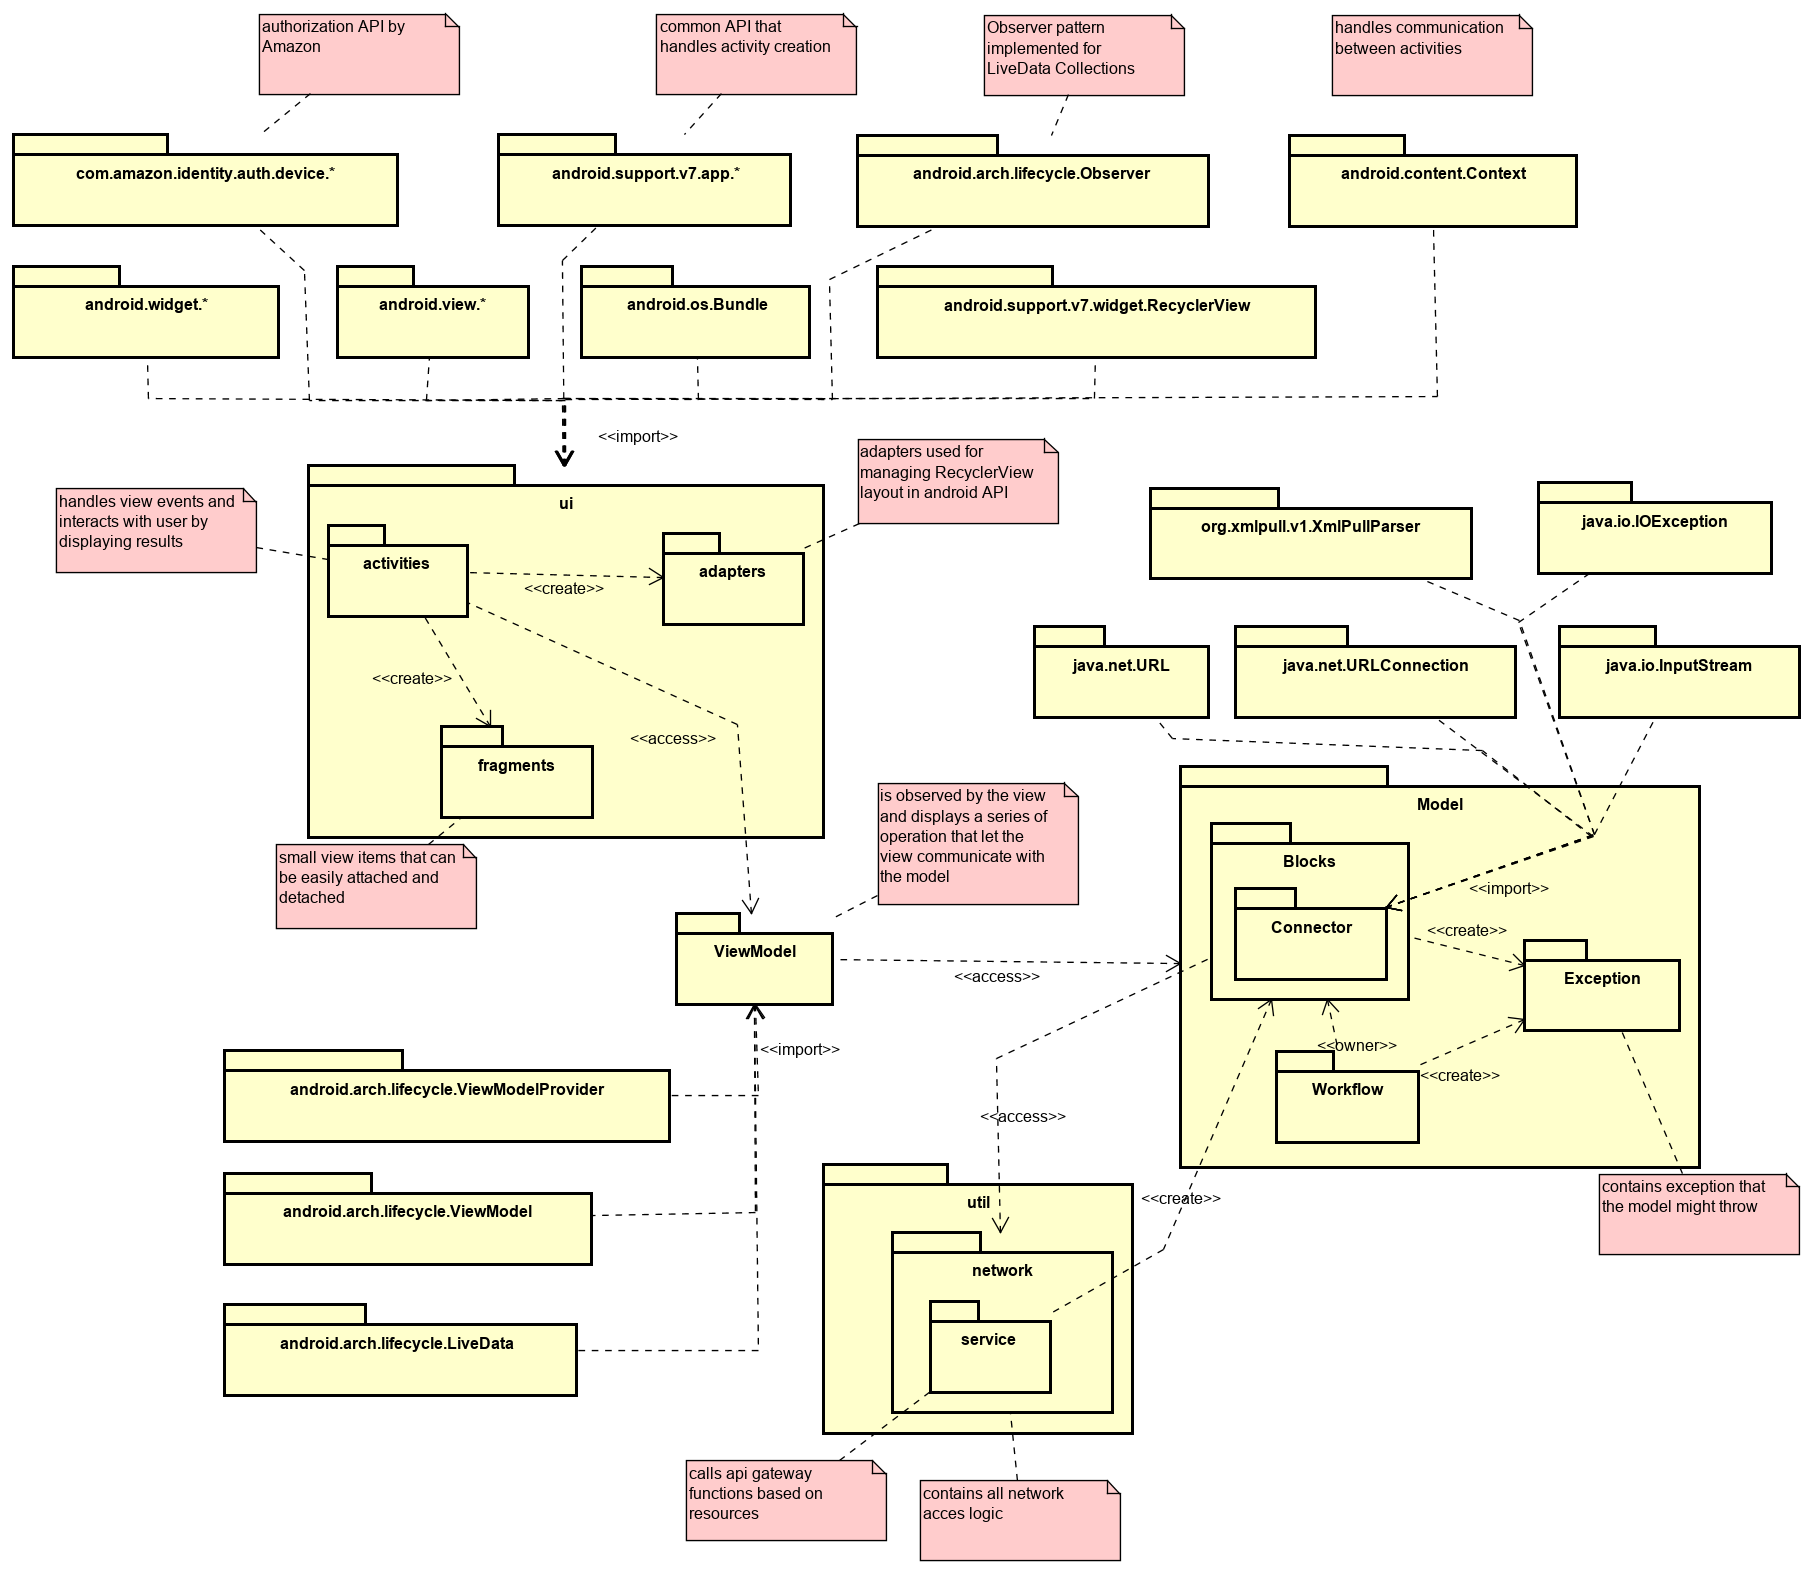
\includegraphics[scale=0.3]{./images/Package.png}
	\caption{\textit{App class diagram - blocks package}}\label{Package}
\end{figure}
\begin{figure} [H]
	\centering
	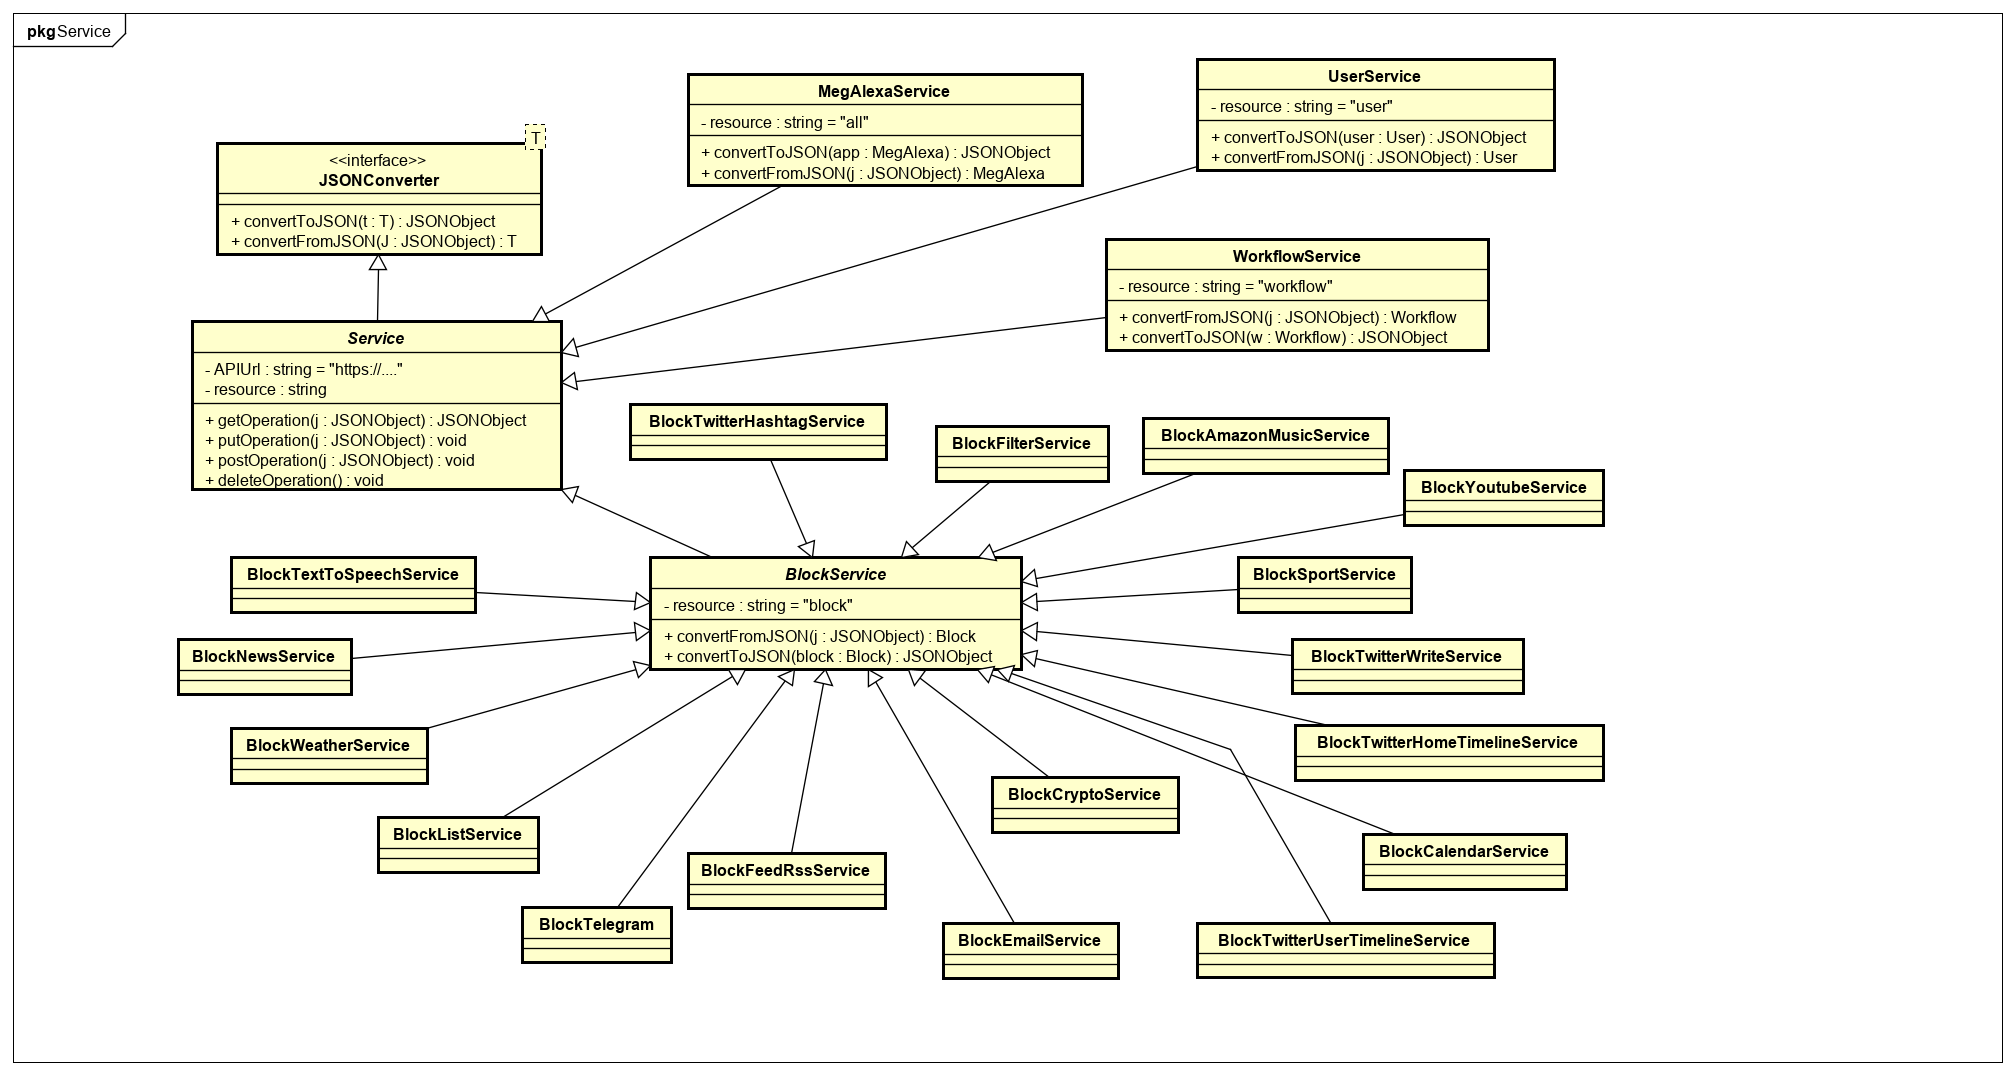
\includegraphics[scale=0.3]{./images/Service.png}
	\caption{\textit{App class diagram - Service}}\label{Service}
\end{figure}
\begin{figure} [H]
	\centering
	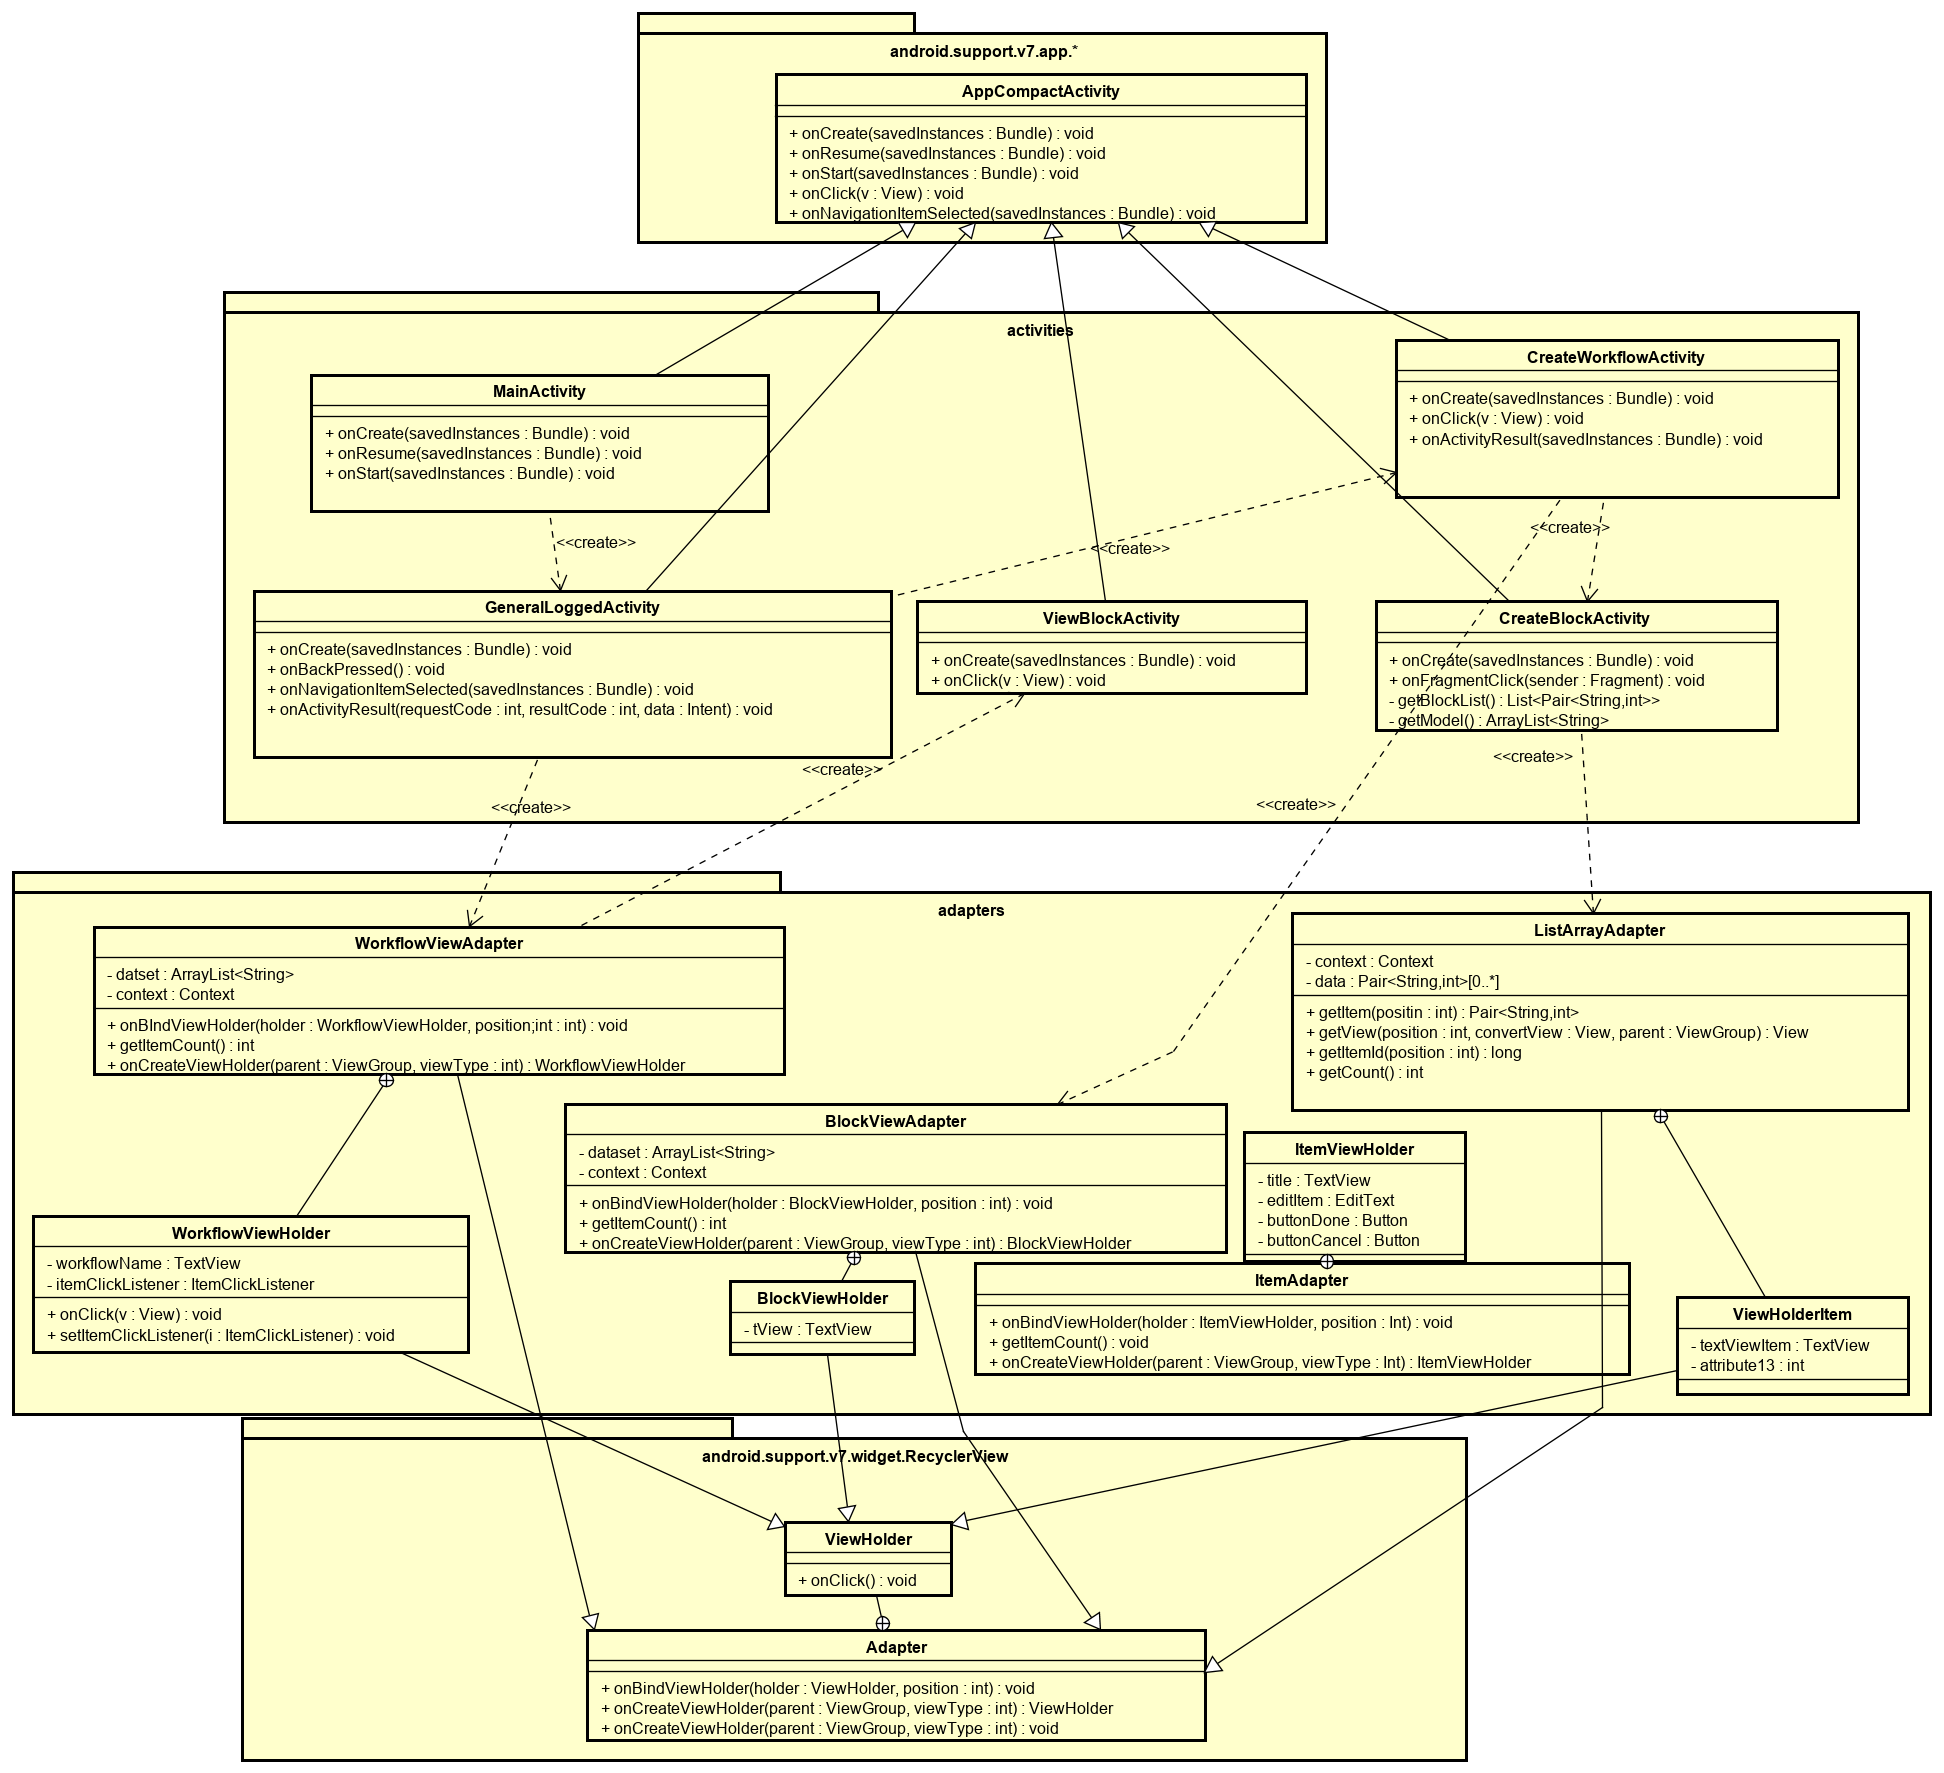
\includegraphics[scale=0.3]{./images/UI.png}
	\caption{\textit{App class diagram - UI}}\label{UI}
\end{figure}

\begin{figure} [H]
	\centering
	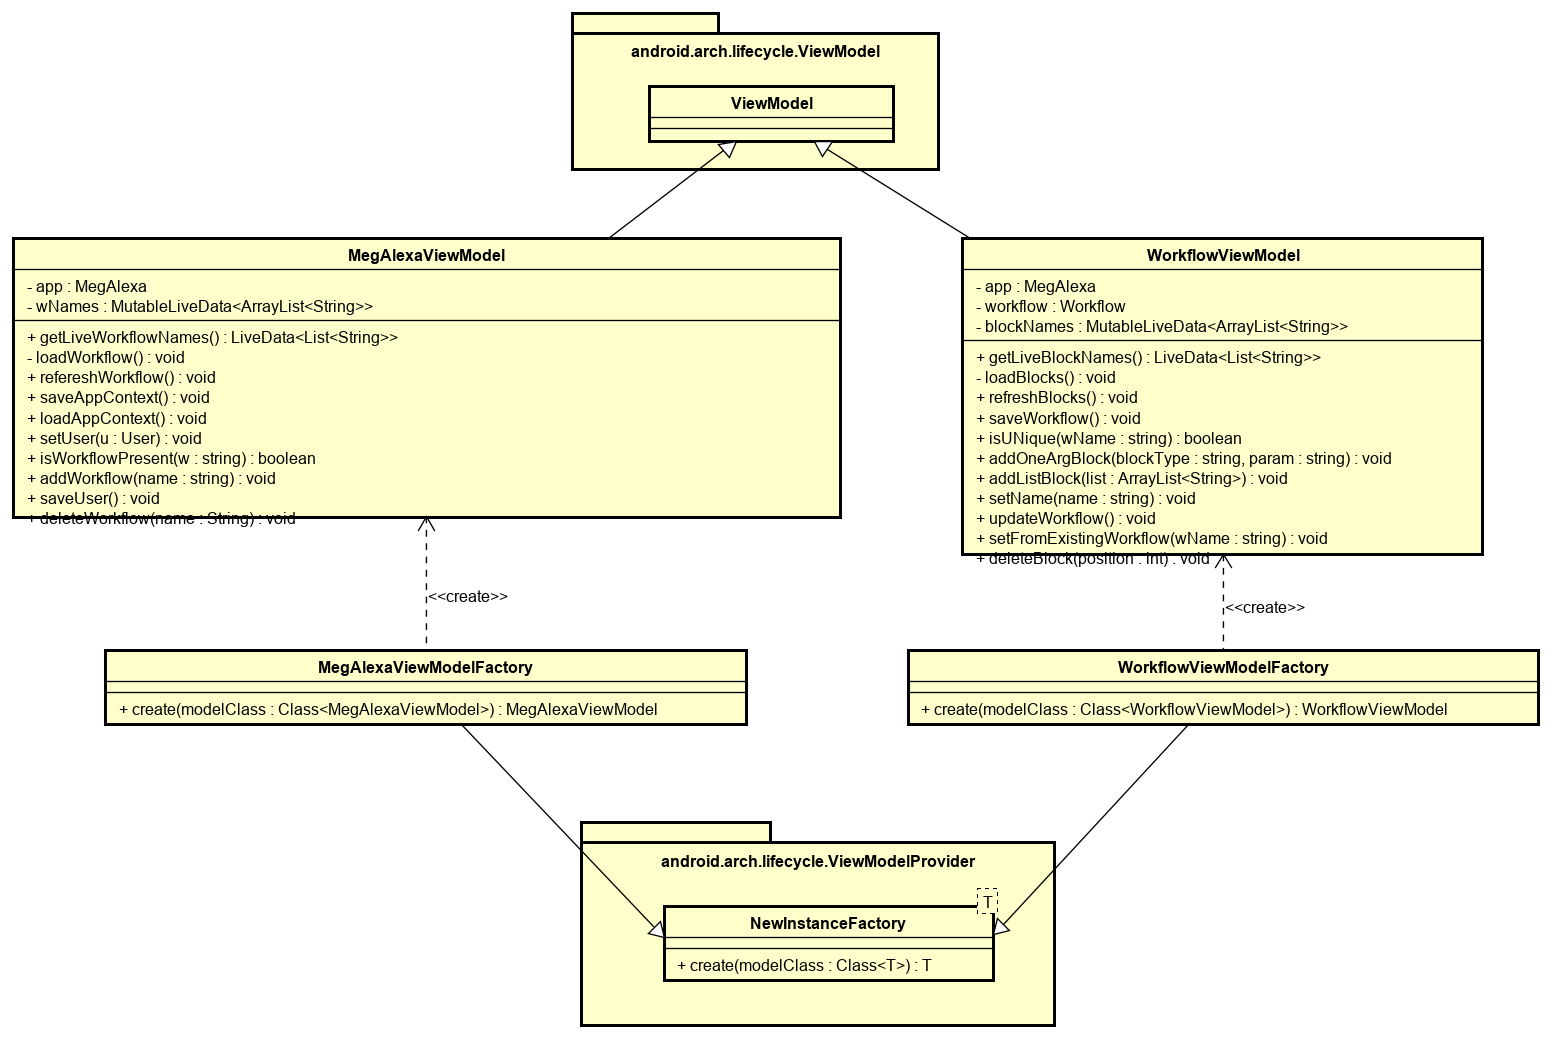
\includegraphics[scale=0.3]{./images/ViewModel.png}
	\caption{\textit{App class diagram - ViewModel}}\label{ViewModel}
\end{figure}

\begin{figure} [H]
	\centering
	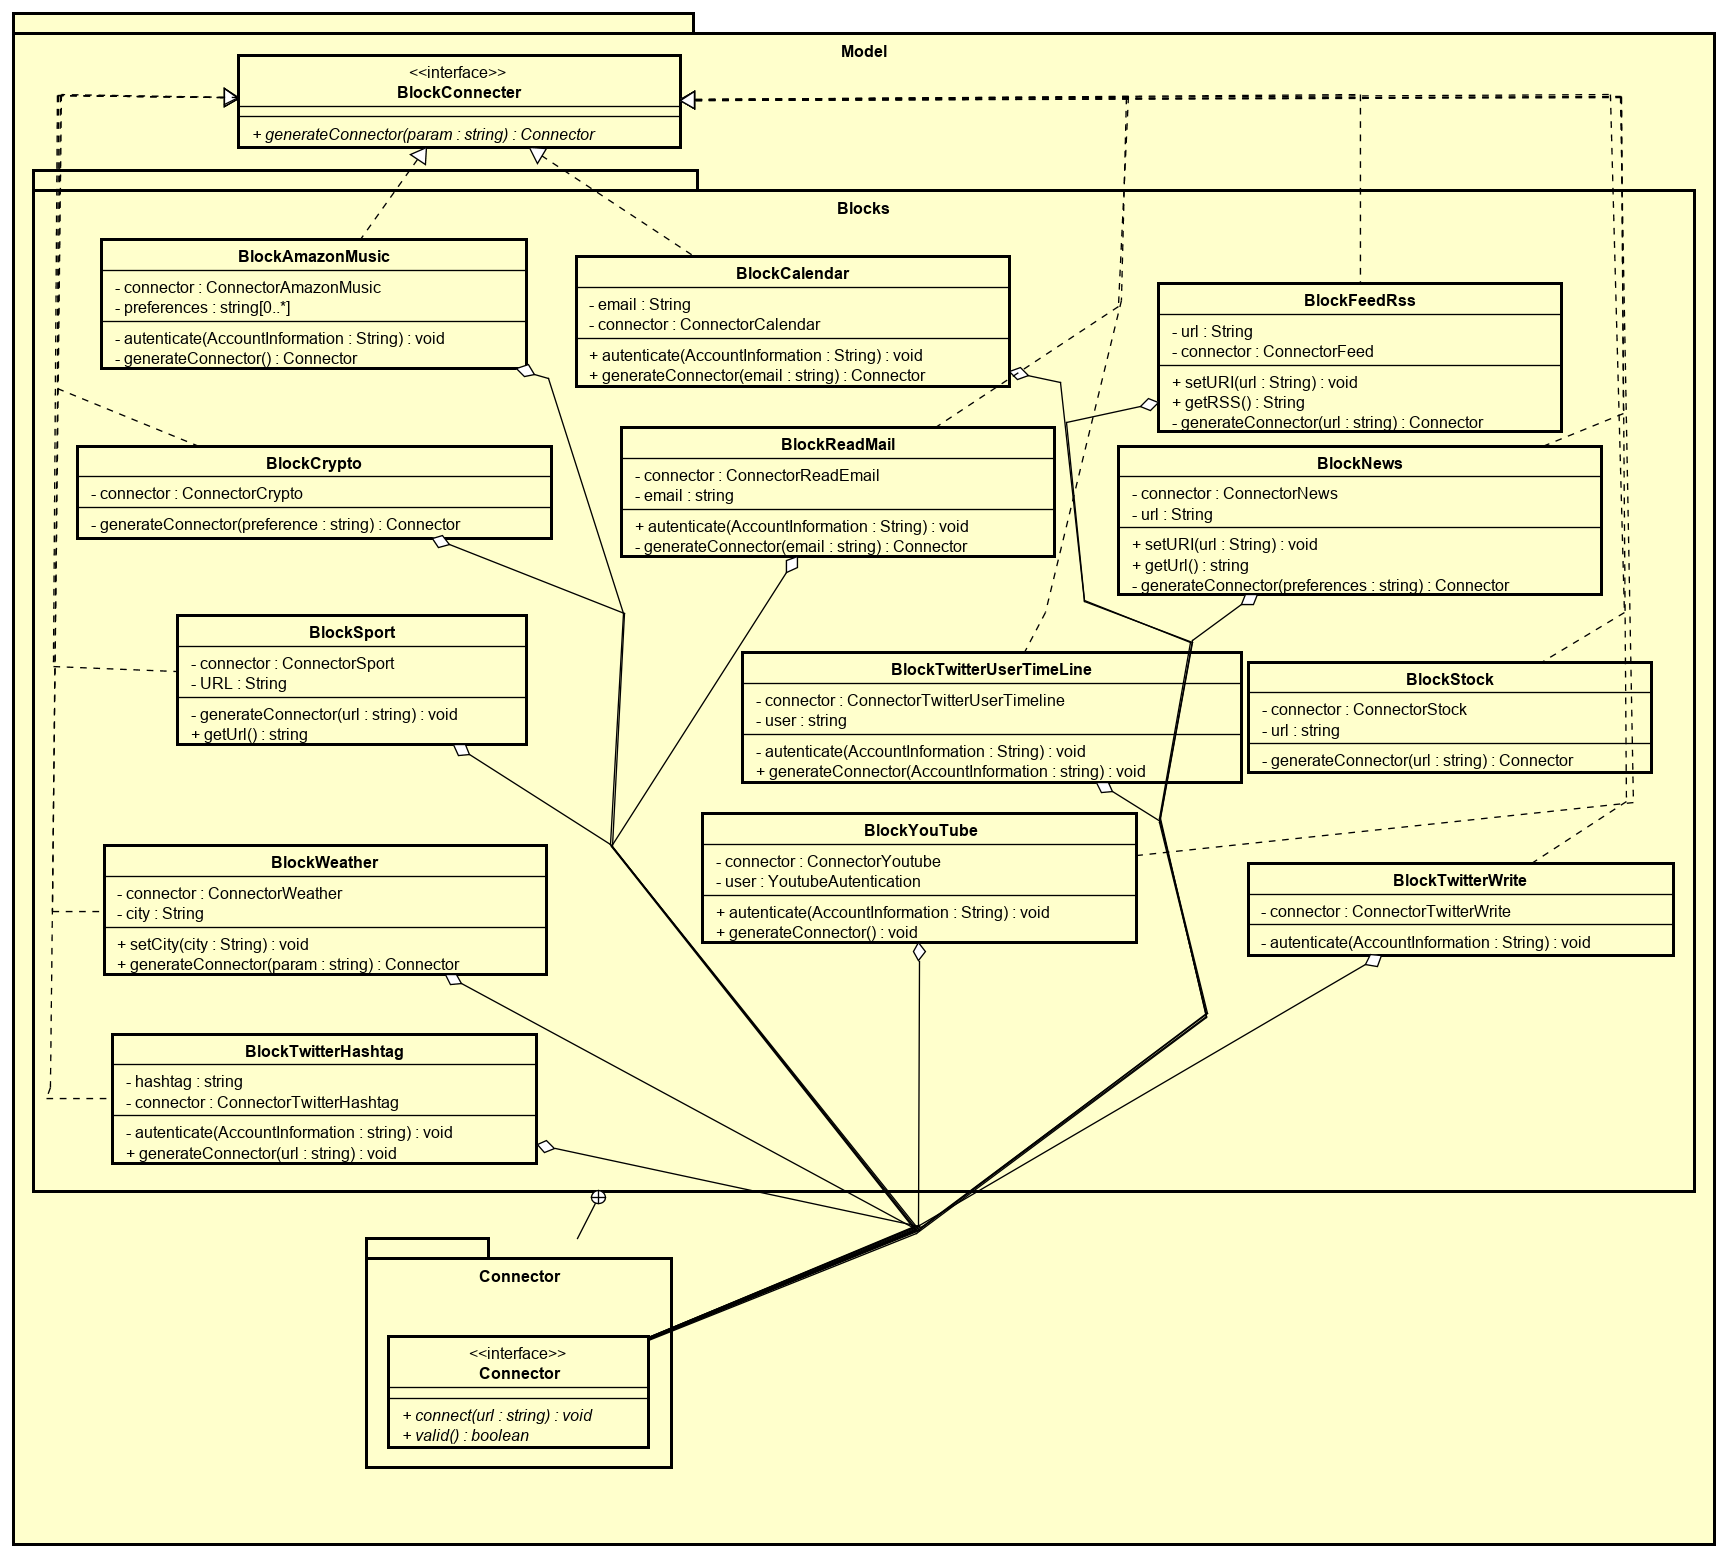
\includegraphics[scale=0.3]{./images/BlockConnection.png}
	\caption{\textit{App class diagram - BlockConnection}}\label{BlockConnection}
\end{figure}

\begin{figure} [H]
	\centering
	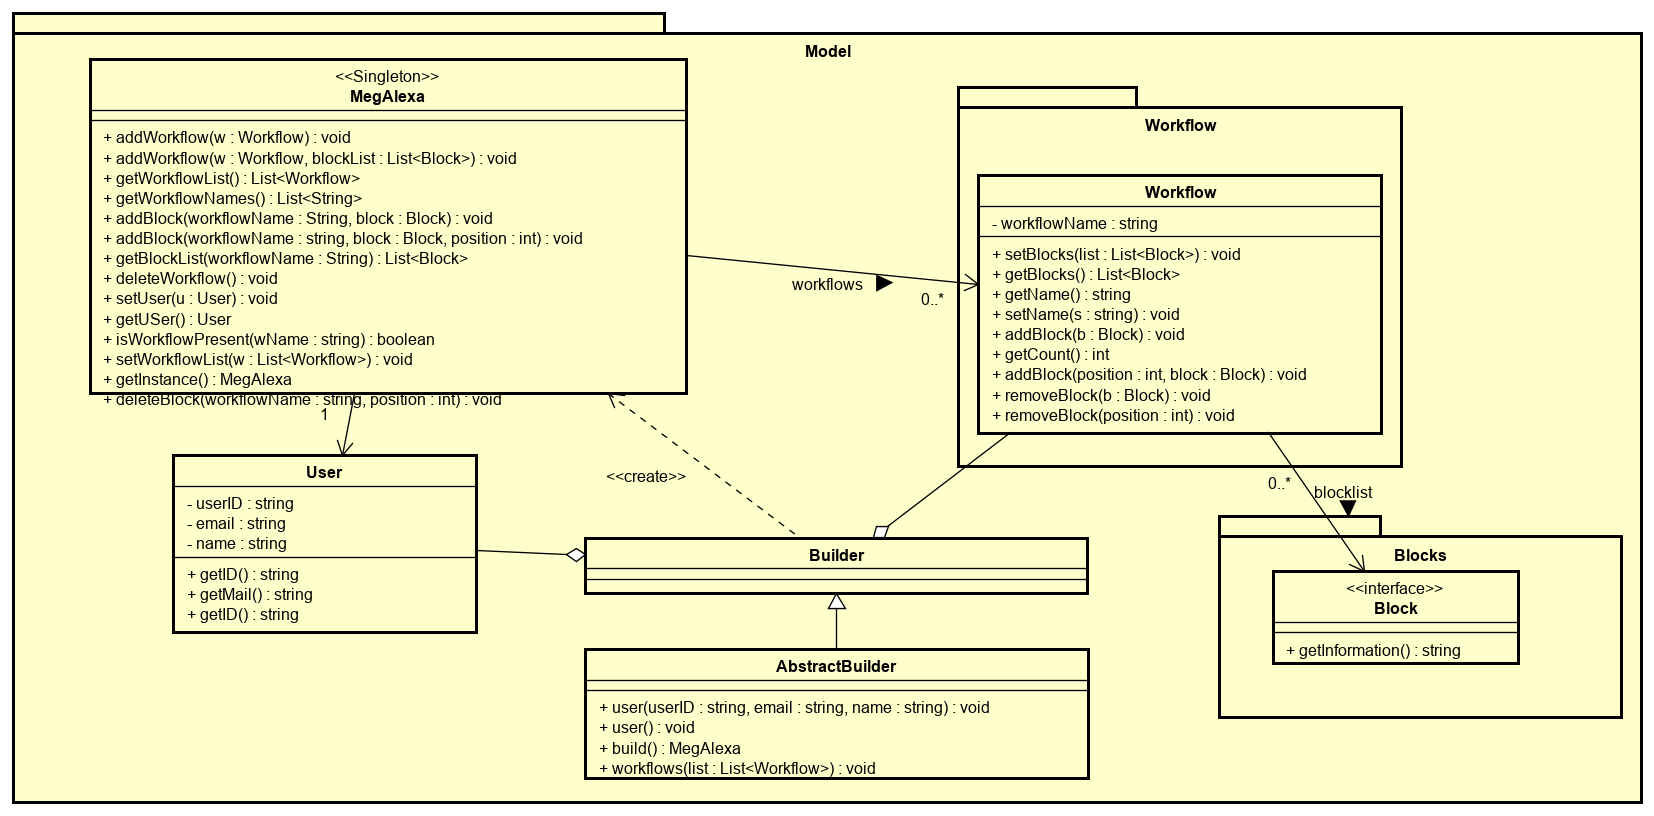
\includegraphics[scale=0.3]{./images/Model.png}
	\caption{\textit{App class diagram - Model}}\label{Model}
\end{figure}
	\chapter{Estensione delle funzionalità}\label{estensione}
In questo capitolo vengono descritti i passaggi per l'estensione del prodotto \textit{MegAlexa}.

\section{Estensione App}
L'estensione della app avviene mediante l'aggiunta di nuovi blocchi.\\
Segue una lista di attività da attuare che descrive i passi da eseguire per un'estensione corretta:

\begin{itemize}
	\item Definire un blocco che derivi dall'interfaccia \texttt{Block} posta nel package \textbf{blocks};
	\item Se il blocco richiede una validazione tramite chiamata esterna, definire un connettore che estenda \texttt{Connector} nel package \textbf{connectors};
	\item Se la chiamata esterna prevede l'utilizzo di una API particolare, definire tali interazioni incapsulandole in una nuova classe da posizionare nel package \textbf{network};
	\item Definire le conversioni da JSON e a JSON dichiarando una nuova classe che derivi da \texttt{BlockService} nel package \textbf{service}, per la comunicazione con \textit{API Gateway$_{G}$};
	\item Ampliare la lista presente in \texttt{CreateBlockActivity} (package \textbf{activities}) in modo che presenti un elemento cliccabile in più;
	\item Definire un widget a scelta (activity o fragment) che rappresenti l'inserimento dei dati da parte dell'utente;
	\item Inserire il listener dell'elemento aggiunto alla lista nel widget appena creato;
	\item Nel caso in cui sia stato creato un fragment ampliare la funzione \textit{onFragmentClick(sender)} in modo che registri e notifichi alle activity interessate le informazioni per l'aggiunta del blocco, in alternativa, se è stata creata una nuova activity, gestire l'interazione con essa mediante le funzioni \textit{startActivityForResult(intent,context)} e \textit{onActivityResult(requestCode,resultCode,data)};
	\item Nella \texttt{CreateWorkflowActivity} e \texttt{ViewBlockActivity}, nelle funzioni \textit{onActivityResult(requestCode,resultCode,data)} 	prelevare i dati passati dalle altre activity e chiamare il viewModel di conseguenza;
	\item Aggiornare il viewModel in modo che supporti l'aggiunta del blocco appena creato.
\end{itemize}



\section{Estensione Skill (lambda)}
La Skill può essere estesa in questi modi:
\begin{itemize}
    \item aggiunta di un nuovo blocco \S\ref{newBlock};
    \item aggiunta di nuove frasi per Alexa \S\ref{newFrasi};
    \item aggiunta di un nuovo metodo d'accesso al database \S\ref{newAccesso};
    \item aggiunta di un nuovo sistema di autenticazione \S\ref{newAuth}.
\end{itemize}
\subsection{Nuovo blocco}\label{newBlock}
Questa sezione verrà redatta quando il prodotto sarà completo.
\subsection{Nuove frasi per Alexa}\label{newFrasi}
Il file phrases-EN.json e phrases-IT.json contengono tutte le frasi personalizzate che Alexa può dire. A ogni parola chiave (uguale per tutte le lingue) sono associate delle frasi (tradotte nella lingua relativa al file).\\
Per inserire una nuova frase, è necessario inserirla nel relativo oggetto associato alla parola chiave. E' importante inserire la frase tradotta per tutti i file phrases-LINGUA.json.\\
Per inserire una nuova parola chiave:
\begin{itemize}
	\item inserire un oggetto contenente come chiave la \textbf{parola chiave} e come contenuto una lista di stringhe, contenenti le frasi;
	\item ripetere l'operazione precedente per ogni lingua;
	\item inserire un nuovo metodo nella classe \textit{PhrasesGenerator.ts}, che ritorna la frase che Alexa deve dire;
	\item l'attributo statico \textbf{jsonPhrases} contiene il file \textit{phrases-LINGUA.json} (la selezione della lingua viene fatta in automatico);
	\item chiamare questo metodo in modo statico dove è necessario.
\end{itemize}
Per inserire una nuova lingua:
\begin{itemize}
	\item inserire un nuovo file \textit{phrases-LINGUA.json}, contenente tutte le parole chiavi presenti negli altri file di configurazione e le relative frasi tradotte;
	\item nel metodo setLanguage aggiungere un case con la nuova lingua.
\end{itemize} 
\subsection{Nuovo metodo d'accesso al database} \label{newAccesso}
Tutti gli accessi al database, per quanto riguarda il download dei workflow, avvengono attraverso la classe \textbf{WorkflowService}, nel metodo \textit{workflowFromDatabase}.\\
\'{E} possibile aggiungere una nuova funzione in \textbf{WorkflowService}, contenente un nuovo metodo d'accesso a un diverso database. Per esempio, può essere fatto attraverso una chiamata HTTP a un servizio REST, oppure usando un web socket. \'{E} necessario che il valore ritornato sia una lista di blocchi.\\
Lo schema del blocco si può trovare nella cartella \textit{JSONconfigurations}, nel file \textit{JSONconfiguration.ts}, con la chiave (\textbf{BlockJSON}).

\subsection{Nuovo sistema di autenticazione}\label{newAuth}
L'autenticazione, nella versione 1.0.0 della skill, avviene solo attraverso Amazon.\\
Il file contenente la richiesta dell'utente (dal Alexa) contiene anche un \textbf{accessToken}. Questo viene utilizzato dalla classe \textbf{User}, dal metodo \textit{credentialsByAccessToken}, per estrarre l'\textbf{AmazonID} dell'utente (lo stesso salvato nel database).\\
Questo sistema è basato su oauth, anche se tutta la parte a basso livello è gestita da Amazon.\\
Per aggiungere un altro sistema di autenticazione basato su oauth:
\begin{itemize}
	\item creare una nuova configurazione Oauth e ottenere i dati d'accesso (URI, clientID, secret...);
	\item aprire il pannello di controllo di Alexa \footnote{\url{https://developer.amazon.com/alexa/console/ask}};
	\item accedere alla skill MegAlexa;
	\item aprire la sezione "account linking";
	\item inserire i dati richiesti, generati da oauth;
	\item nella skill MegAlexa, modificare la funzione \textit{credentialsByAccessToken}, nella classe \textbf{User}, così che sia compatibile con il nuovo servizio (ciò che cambia sarà l'ID e la chiamata GET per ottenerlo).
\end{itemize}
	\label{LastPage}
\end{document}